\chapter{Le paradoxe de la sphère de Hausdorff}
\section{Introduction.}
\noindent
Le but de ce chapitre est de démontrer le paradoxe de Hausdorff, qui constitue un premier exemple du paradoxe de Banach-Tarski; Le paradoxe lui même s'appuie sur cet exemple.

\begin{theorem}(Paradoxe de Hausdorff)
  \hfill

  La sphère unitée $\mathrm{S}^2$ peut être découpée en un nombre fini de parties disjointes, $A_1,A_2,...,A_n$, tels qu'il existe des isométries positives $\varphi_1, \varphi_2, ..., \varphi_n$ telles que $\underset{1\le i\le n}{\cup} \varphi(A_i)$ est deux copies de $\mathrm{S}^2$.
  \label{But}
\end{theorem}
\noindent
On va se baser dans ce chapitre sur la référence \cite{cite1}.
\section{Notations.}
\noindent
Dans tout ce chapitre, $\mathrm{E}$ est un espace vectoriel euclidien orienté de dimension $3$, rapporté à une base $\mathcal{B}$ orthonormée directe. Le produit scalaire de deux vecteurs $u$ et $v$ est noté $\langle u, v \rangle$. Les déplacements de $E$ sont les rotations et les translations.(c'est à dire des isométries positives)\\
Soit $\Omega$ un ensemble quelquonque non vide. $A$ et $B$ étant deux sous-ensembles de $\Omega$, on note $A$ \textbackslash $B$
l'intersection de $A$ et du complémentaire de $B$; en d'autres termes :
$$A \text{\textbackslash} B = \{x \in \Omega \text{ | } x \in A \text{ et } x \notin B \}$$
$\mathfrak{S}(\Omega)$ désigne le groupe des bijections de $\Omega$ dans lui-même.
Soit $f \in \mathfrak{S}(\Omega)$, si $A$ est un sous-ensemble de $\Omega$, on notera $f(A)$ le sous-ensemble de $\Omega$ dont les éléments sont dans les
images des éléments de $A$ : $$f(A) = \{ y \in \Omega \text{ | } \exists x \in A \text{ tq } f(x)=y \}$$
\section{Préliminaires.}
\noindent
Avant de commencer on va rappeller quelques résultats sur les fonctions de $\mathfrak{S}(\Omega)$ qui nous seront utiles par la suite.
\begin{lemma}\label{lemme 1}
Soient $\Omega \ne \emptyset$, $A$ et $B$ deux sous-ensembles de $\Omega$, et $f \in \mathfrak{S}(\Omega)$, on a alors :
\begin{enumerate}
\item \label{1} $f(A)= \emptyset \Leftrightarrow  A=\emptyset$
\item \label{2}$A, B \subset \Omega \Rightarrow (A \subset B \Leftrightarrow f(A) \subset f(B))$
\item \label{3} Si $(A_i)_{i \in I}$ est une famille de sous-ensembles de $\Omega$ indexée par l'ensemble $I$, alors:
$$ f\big(\bigcup_{i \in I} A_i \big)= \bigcup_{i \in I} f(A_i) $$
\item \label{4} Si $(A_i)_{i \in I}$ est une famille de sous-ensembles de $\Omega$ indexée par l'ensemble $I$, alors:
$$ f\big(\bigcap_{i \in I} A_i \big)= \bigcap_{i \in I} f(A_i) $$
\item \label{5} $f(A \text{\textbackslash} B) = f(A) \text{\textbackslash} f(B)$
\end{enumerate}

\end{lemma}

\begin{proof}[Démonstration]\label{demo1}
\hfill

\noindent
Les trois premières affirmations sont vraies pour toutes les applications, et on les admet. Démontrons les deux dérnières affirmations :
\begin{itemize}
\item  Pour \ref{4}, l'implication directe est toujours vérifiée :
  \begin{align*}
    y \in f\big(\bigcap_{i \in I} A_i \big) &\Rightarrow \exists x \in \bigcap_{i \in I} A_i, y=f(x) \Rightarrow y \in \bigcap_{i \in I} f(A_i)
  \end{align*}
  Pour l'implication réciproque on a besoin de l'injectivité de $f$ :
  \begin{align*}
    y \in \bigcap_{i \in I} f(A_i) &\Rightarrow \forall i \in I, \exists y' \in f(A_i), y=y'
    \Rightarrow \forall i \in I, \exists x_i \in A_i, y=f(x_i)\\
    &\Rightarrow \forall i \in I, \exists x_i \in A_i, y=f(x_i) \text{ et } x_i = x_j \forall i,j \\
    &\Rightarrow \exists x \in \bigcap_{i \in I}A_i, y=f(x) \Rightarrow y \in f\big(\bigcap_{i \in I}A_i\big)
  \end{align*}
\item  Pour \ref{5} l'inclusion réciproque est toujours vraie :
  \begin{align*}
    y \in f(A) \text{\textbackslash} f(B) &\Rightarrow \exists x \in A, y=f(x) \text{ et } \forall x' \in B, y \neq  f(x')\\
      &\Rightarrow \exists x \in A \text{\textbackslash} B, y=f(x) \Rightarrow y \in f(A \text{\textbackslash} B)
  \end{align*}
  Pour l'inclusion directe on a besoin de l'injectivité de $f$ :
  \begin{align*}
    y \in f(A \text{\textbackslash} B) &\Rightarrow \exists x \in A\text{\textbackslash} B, y=f(x) \Rightarrow y \in f(A) \text{ et } \forall x' \in B, y \neq f(x') \Rightarrow  y \in f(A) \text{\textbackslash} f(B)
  \end{align*}
\end{itemize}
\end{proof}
\begin{Cor}\label{lemme 2}
  Sous les conditions du \hyperref[lemme 1]{Lemme 1} :
  $$(A_i)_{i \in I} \text{ est une partition de } \Omega \Leftrightarrow  (f(A_i))_{i \in I} \text{ est une partition de } \Omega$$
\end{Cor}
\begin{proof}[Démonstration]\label{demo2}
  Ceci découle de \ref{1}, \ref{3} et \ref{4} :
  \begin{align*}
    (A_i)_{i \in I} \text{ est une partition de } \Omega  &\Leftrightarrow  \left\{
                                                                                \begin{array}{ll}
                                                                                    \forall i \in I, A_i \neq \emptyset \\
                                                                                    \bigcup_{i \in I} A_i = \Omega \\
                                                                                    \forall (i,j), i\neq j \Rightarrow A_i \cap A_j = \emptyset
                                                                                \end{array}
                                                                            \right. \\
  &\Overset{\underset{f}{\Rightarrow}}{\overset{f^{-1}}{\Leftarrow}}  \left\{
                         \begin{array}{ll}
                             \forall i \in I, f(A_i) \neq f(\emptyset) = \emptyset \\
                             \bigcup_{i \in I} f(A_i)=f(\bigcup_{i \in I} A_i) = f(\Omega) = \Omega  \\
                             \forall (i,j), i\neq j \Rightarrow f(A_i \cap A_j)= f(A_i) \cap f(A_j) = \emptyset
                         \end{array}
                     \right.
  \end{align*}
\noindent
L'implication réciproque se démontre en composant avec $f^{-1}$ $\text{qui a les mêmes propriétées que $f$}$.
\end{proof}

\section{Schéma de la démonstration du paradoxe de Hausdorff.}
\noindent
Dans cette section on présente une vue d'ensemble de la démonstration du paradoxe de Hausdorff, avant de s'atteler aux détails de la démonstration.
Les raisonnements de cette section sont inspirés de la réference \cite{cite2}.
Avant de lister les étapes qu'on va suivre, on a tout d'abord besoin de quelques définitions
\begin{definition}
  Un alphabet dans un ensemble $\mathrm{G}$ est un ensemble fini et non vide d'éléments distincts de $\mathrm{G}$.
\end{definition}
\begin{definition}
  Un mot défini dans un alphabet $\mathcal{A}$ est une suite finie d'éléments de $\mathcal{A}$.\\ La longueur d'un tel mot est le nombre d'éléments dans la suite.
\end{definition}
\begin{definition}
Un mot est dit réduit s'il ne contient pas deux éléments consécutifs qui soient inverses l'un de l'autre.
\end{definition}
\begin{definition}
  On dit que deux éléments $\theta$ et $\varphi$ d’un groupe $\mathrm{G}$ sont indépendants si pour tout mot réduit de longueur $n\ge 2$, $(g_1, ..., g_n)$ dans l'alphabet $\mathcal{A} = \{\theta, \varphi, \theta^{-1}, \varphi^{-1}\}$ on a que $g_1...g_n \ne 1_\mathrm{G}$.
\end{definition}
% \begin{definition}
% On dit que deux éléments $\theta$ et $\varphi$ d’un groupe $\mathrm{G}$ sont indépendants si les éléments $\theta$, $\varphi$, $\theta^{-1}$ et $\varphi^{-1}$ de $\mathrm{G}$ sont tous distincts et si pour tout $n > 2$ et pour toute liste d'éléments $(g_1, ..., g_n)$ de $\mathrm{G}$ tous égaux à $\theta$, $\varphi$, $\theta^{-1}$ ou $\varphi^{-1}$, il est impossible d’avoir $g_1...g_n = 1$ si $g_ig_{i+1} \neq 1$ pour $i = 1, ..., n-1$.
% \end{definition}
\begin{definition}
Si un groupe $\mathrm{G}$ est engendré par deux éléments $\theta$ et $\varphi$ indépendants, on dit
que $\mathrm{G}$ est librement engendré par $\theta$ et $\varphi$. $\mathrm{G}$ est alors appelé un groupe libre de rang $2$.
\end{definition}
\noindent
Pour démontrer notre \hyperref[But]{théorème} on va procéder comme suit
\subsection{Première étape de la démonstration .}
% %%%%%%%%%%%%%%%%%%%%%%%%%%%%%%%%%%%%%%%%%%%%%%%%%%%%%%%%%%%%%%%%%%%%%%%%%%%%%%%%%%%%%%%%%%%%%%%%%%%%%%%%%%%%%%%%%%%%%%%%%%%%
\noindent
 On va construire un groupe libre de rang $2$ contenu dans $\mathcal{SO}(3)$ et engendré par deux éléments $\theta$ et $\varphi$. L'interet de cette construction est que ce groupe peut être représenté par la fractale suivante qu'on appelle le graphe de Cayley:
  \begin{figure}[h]
      \centering
      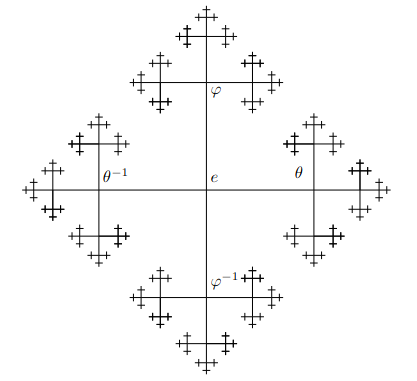
\includegraphics[scale=0.5]{./images/bt.png}
      % \caption{Une représentation graphique d'un groupe libre de rang 2}
      \label{fig1}
  \end{figure}\\
  \noindent
  Dans cette représentation, les éléments de $\mathrm{G}$ sont les intersections des différents segments, et sont répartis de la manière suivante :
  \begin{itemize}
    \item L'élément neutre est le centre de la fractale.
    \item Pour multiplier un élément par $\theta$ à gauche on se déplace (dans la fractale) à partir de cet élément vers la gauche.
    \item Pour multiplier un élément par $\theta^{-1}$ à gauche on se déplace (dans la fractale) à partir de cet élément vers la droite.
    \item Pour multiplier un élément par $\varphi$ à gauche on se déplace (dans la fractale) à partir de cet élément vers le haut.
    \item Pour multiplier un élément par $\varphi^{-1}$ à gauche on se déplace (dans la fractale) à partir de cet élément vers le bas.
  \end{itemize}
  On note $\mathrm{L}(\sigma)$ la composante connexe de la fractale privé de l'élément neutre, qui contient $\sigma$, pour \\$\sigma \in \{\theta, \theta^{-1}, \varphi, \varphi^{-1}\}$.
  Si on multiplie à gauche par $\theta$ la composante $\mathrm{L}(\theta^{-1})$, on obtient la réunion des points des trois composantes $\mathrm{L}(\varphi^{-1})$, $\mathrm{L}(\theta^{-1})$ et $\mathrm{L}(\varphi)$, plus l'élément neutre.\\
\\
  \begin{minipage}{0.1\textwidth}
  \centering
  $\mathrm{L}(\theta^{-1}) =$
  \end{minipage}%
  \begin{minipage}{0.25\textwidth}
  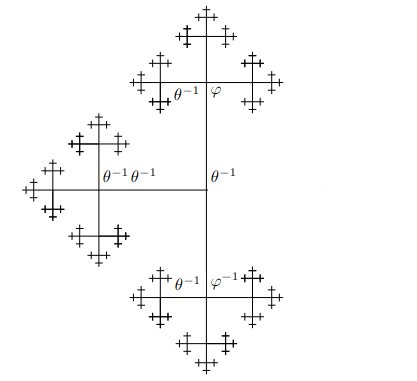
\includegraphics[scale=0.4]{./images/btt.png}
  \end{minipage}%
  \begin{minipage}{0.1\textwidth}
  \centering
  $\overset{\theta}{--\longrightarrow}$ %$\theta\mathrm{L}(\theta^{-1})=$
  \end{minipage}%
  \begin{minipage}{0.25\textwidth}
  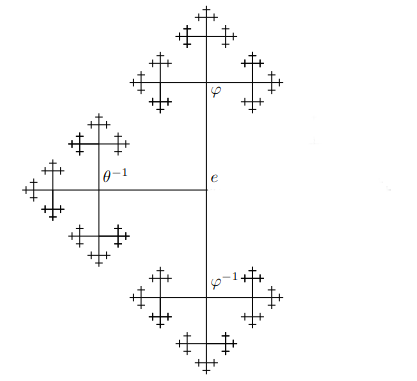
\includegraphics[scale=0.4]{./images/bttt.png}
  \end{minipage}%
  \begin{minipage}{0.3\textwidth}
  \centering
  $=\{e\}\cup \mathrm{L}(\theta^{-1}) \cup \mathrm{L}(\varphi^{-1}) \cup \mathrm{L}(\varphi)$
  \end{minipage}%
\\
\bigskip

\noindent
  De même si on multiplie à gauche par $\varphi$ la composante $\mathrm{L}(\varphi^{-1})$, on obtient les trois composantes $\mathrm{L}(\varphi^{-1})$, $\mathrm{L}(\theta^{-1})$ et $\mathrm{L}(\theta)$, plus l'élément neutre.
  En d'autres termes :
  $$\mathrm{G} = \mathrm{L}(\theta)\cup\theta\mathrm{L}(\theta^{-1})= \mathrm{L}(\varphi)\cup\varphi\mathrm{L}(\varphi^{-1})$$
  % On a pu alors construire $\mathrm{G}$ à partir de parties disjointes dont la réunion est strictement incluse dans $\mathrm{G}$.

  \begin{remarkk}\label{remarque2}
    Le fait que le groupe $G$ est libre implique que ses éléments s'écrivent de manière unique comme mot de l'alphabet $\{\theta, \varphi, \theta^{-1}, \varphi^{-1}\}$; en d'autres mots, on ne peut jamais tomber sur un même élément en partant dans deux chemins différents dans la fractale, et en particulier les réunions ci-dessus sont disjointes.
  \end{remarkk}
  \noindent
  Le groupe $\mathrm{G}$ a donc la propriété d'être décomposable en parties disjointes, $\mathrm{L}(\varphi^{-1})$, $\mathrm{L}(\varphi)$, $\mathrm{L}(\theta^{-1})$ et $\mathrm{L}(\theta)$ telles qu'on peut reconstruire $\mathrm{G}$ soit à partir des deux premières, ou à partir des deux dernières parties.
\subsection{Deuxième étape de la démonstration .}\label{2.}
Après, on va éssayer d'importer cette propriété de $\mathrm{G}$ à $\mathrm{S}^2$ en écrivant $\mathrm{S}^2$ comme réunion d'orbites de $\mathrm{G}$. Ce programme sera mis en difficulté par le fait que la sphère $\mathrm{S}^2$ contient des éléments qui peuvent être fixés par des éléments de $\mathrm{G}$, c.à.d que pour certains $x$ l'application $G \rightarrow S^2$ donnée par $g \rightarrow g(x)$ ne sera pas injective.
  On va donc dans un premier temps travailler avec l'ensemble $$\mathrm{X} = \mathrm{S}^2 - \{s \in \mathrm{S}^2 \mid \exists g \in \mathrm{G}, g(x) = x\}$$ de sorte que l'action de $\mathrm{G}$ sur $\mathrm{X}$ soit libre, i.e :
  \begin{align*}
 g_X \colon X &\to X\\
 x &\mapsto g(x).
\end{align*}
est bijective puisque $g$ est inversible et que :
  \begin{align*}
  \phi \colon \mathrm{G} &\to \mathfrak{S}(X)\\
  g &\mapsto g_X.
\end{align*}
est un homomorphisme qui vérifie que pour tout $x\in X$, $g(x) = x \Rightarrow g = \mathrm{Id_E}$.\\
$G$ a la propriété d'être dans un certain sens algébriquement équidécomposable à deux copies de lui même, on va montrer donc qu'on peut importer cette propriété de $\mathrm{G}$ à $\mathrm{X}$. Pour cela on va procéder comme suit
\begin{itemize}
  \item Dans chaque $G$-orbite de $X$ on va sélectionner un seul élément, pour garantir une unicité des éléments de $X$ après l'action de $G$. Cette selection sera faite en utilisant \hyperref[axiome]{l'axiome du choix}, $M$ sera l'union de ces choix.
  \item On représente donc $\mathrm{X}$ par la même fractale qu'avant, en remplaçant chaque élément $g \in \mathrm{G}$ par l'ensemble $g(\mathrm{M}) \subset \mathrm{X}$. On peut alors répéter le même raisonnement que pour $\mathrm{G}$; en divisant chaque $G$-orbite de la même façon que pour $G$, pour construire $\mathrm{X}$ à partir de parties disjointes dont la réunion est strictement incluse dans $\mathrm{X}$. On dit que $\mathrm{X}$ est \hyperref[ed]{équidécomposable} à deux copies de $\mathrm{X}$.
\end{itemize}
 % En effet, pour garantir une unicité des éléments de $\mathrm{X}$ après l'action de $\mathrm{G}$, on va identifier les éléments $a$ et $b$ de $\mathrm{X}$ qui vérifient $g(a)=h(b)$ pour $g, h \in \mathrm{G}$, et pour cela on va prendre un seul élément de chaque orbite, et donc on utilise \hyperref[axiome]{l'axiome du choix} pour construire un ensemble $\mathrm{M}$ qui contient un représentant de chaque orbite, alors l'ensemble $\mathrm{X}$ peut être représenté par la même fractale qu'avant, sauf à la place de chaque $g \in \mathrm{G}$ on aura $g(\mathrm{M})$, et on peut alors répéter le même raisonnement que pour $\mathrm{G}$ pour construire $\mathrm{X}$ à partir de parties dont l'union est strictement incluse dans $\mathrm{X}$.\\
%   \item \label{2.} Après, on va construire un sous-ensemble $\mathrm{X}$ de $\mathrm{S}^2$ qui à la fois peut être découpée en parties, et réarangée (après rotations et translations) pour obtenir $\mathrm{S}^2$, et tel que l'action de $\mathrm{G}$ sur $\mathrm{X}$ soit libre, i.e :
%   \begin{align*}
%  g_X \colon X &\to X\\
%  x &\mapsto g(x).
% \end{align*}
% est bien définie $\forall g \in \mathrm{G}$ (et même bijective puisque $g$ est inversible) et que :
%   \begin{align*}
%   \phi \colon \mathrm{G} &\to \mathfrak{S}(X)\\
%   g &\mapsto g_X.
% \end{align*}
% soit un homomorphisme qui vérifie que pour tout $x\in X$, $g(x) = x \Rightarrow g = \mathrm{Id_E}$,
%   pour qu'on puisse faire passer la propriété de $\mathrm{G}$ à $\mathrm{X}$.\\ En effet, en utilisant la
%   \hyperref[remarque2]{Remarque 1}, on aurra besoin pour avoir une sorte d'unicité après l'action de $\mathrm{G}$ sur $\mathrm{X}$,
%   qu'aucun élément de $\mathrm{X}$ ne se répète après composition par un élément de $\mathrm{G}$ i.e ,\\ ($\forall x \in X$, $g(x) = x \Rightarrow g = \mathrm{Id_E}$) , de plus il nous faut identifier les éléments $a$ et $b$ de $\mathrm{X}$ qui vérifient $g(a)=h(b)$ pour $g, h \in \mathrm{G}$, et pour cela il nous faut prendre qu'un seul élément de chaque orbite, et donc on utilise l'axiome du choix pour construire un ensemble $\mathrm{M}$ qui contient un représentant de chaque orbite, alors l'ensemble $\mathrm{X}$ peut être représenté par la même fractale qu'avant, sauf à la place des $g$ il y aura des $g(\mathrm{M})$, et on peut alors répéter le même raisonnement que pour $\mathrm{G}$ pour construire $\mathrm{X}$ à partir de parties dont l'union est strictement incluse dans $\mathrm{X}$.\\
%
%   \begin{remarkk}\label{remarque3}
%     Remarquons ici que pour que ce résonnement soit vrai, il ne faut pas que tous les éléments de $\mathrm{X}$ soient regroupés dans le centre de la fractale, c.à.d il faut que $\mathrm{M} \ne \mathrm{X}$, i.e : $\exists x \in \mathrm{X}, \exists g \in G$ tel que $g(x) \ne x$, ce qui est vérifié car l'action est libre.
%   \end{remarkk}
\subsection{Troisième étape de la démonstration .}
\noindent
 En fin, on va montrer que $\mathrm{S}^2$ est \hyperref[ed]{équidécomposable} à $\mathrm{X}$, et donc équidécomposable à la réunion de deux copies de $\mathrm{X}$, et que chaque copie de $\mathrm{X}$ est équidécomposable à $\mathrm{S}^2$, pour conclure que $\mathrm{S}^2$ est équidécomposable à deux copies de $\mathrm{S}^2$.
  % \item En fin, il suffit de transformer $\mathrm{S}^2$ en $\mathrm{X}$, transformer $\mathrm{X}$ en "deux $\mathrm{X}$", et en fin transformer chaqu'un des $\mathrm{X}$ en $\mathrm{S}^2$, (transformer signifie : découper et réaranger après rotations et translations).

%%%%%%%%%%%%%%%%%%%%%%%%%%%%%%%%%%%%%%%%%%%%%%%%%%%%%%%%%%%%%%%%%%%%%%%%%%%%%%%%%%%%%%%%%%%%%%%%%%%%%%%%%%%%%%%%%%%%%%%%%%%%%%%%%%%%%%%%%%%%%
\begin{remarkk}\label{remarque1}
  Un groupe libre de rang $2$ ne peut pas être abélien.($g_1g_2 = g_2g_1 \Rightarrow g_1^{-1}g_2^{-1}g_1g_2=1_G$, ce qui contredit la définition d'un groupe libre).
\end{remarkk}
\noindent
On va chercher donc à construire un sous-groupe libre de rang $2$, $\mathrm{G} = \langle \rho, \tau \rangle$, dans $\mathcal{SO}(3)$. D'après la \hyperref[remarque1]{Remarque 2}, il faut que $\mathrm{G}$ soit non abélien, ceci nous conduit à étudier la commutativité de deux rotation de $\mathrm{E}$.

\section{Rotations d'un espace vectoriel euclidien orienté de dimention 3 .}
\begin{prop}\label{prop1}
  Soit $\rho_1$ et $\rho_2$ deux rotations vectorielles $\neq \mathrm{Id_E}$ de $\mathrm{E}$, alors :
  $$\rho_1, \rho_2 \text{ commutent } \Leftrightarrow (\text{$\rho_1$ et $\rho_2$ ont même axe ou sont des demi-tour d'axes orthogonaux})$$
\end{prop}
\begin{proof}
\hfill
\begin{itemize}
  \item On commence par l'implication réciproque, et on suppose dans un premier temps que $\rho_1$ et $\rho_2$ sont des rotations  d'angles $\alpha_1$ et $\alpha_2$ respectivement autour de la droite $D$ dirigée et orientée par un vecteur unitaire $\omega$, qu'on peut le compléter en une base orthonormée $B = (\omega, e, u)$.\\ Les matrices de $\rho_1$ et $\rho_2$ dans cette base sont:
  \[
  \mathrm{P}_1=
  \begin{pmatrix}
  1 & 0 & 0\\
  0 & \cos(\alpha_1) & -\sin(\alpha_1) \\
  0 & \sin(\alpha_1) & \cos(\alpha_1)
  \end{pmatrix}
  \text{ et }
  \mathrm{P}_2=
  \begin{pmatrix}
  1 & 0 & 0\\
  0 & \cos(\alpha_2) & -\sin(\alpha_2) \\
  0 & \sin(\alpha_2) & \cos(\alpha_2)
  \end{pmatrix}
  \]
  Alors il est clair que :
  \[
   \mathrm{P}_1 \mathrm{P}_2=\mathrm{P}_2 \mathrm{P}_1=
   \begin{pmatrix}
   1 & 0 & 0\\
   0 & \cos(\alpha_1+\alpha_2) & -\sin(\alpha_1+\alpha_2) \\
   0 & \sin(\alpha_1+\alpha_2) & \cos(\alpha_1+\alpha_2)
   \end{pmatrix}
   \]
   qui est la rotation d'axe $D$ qui est dirigée et orientée par $\omega$, d'angle $\alpha_1 + \alpha_2$.
  %
  \tdplotsetmaincoords{60}{110}

  \begin{center}
  \begin{tikzpicture}[tdplot_main_coords, scale = 2.5]
  \coordinate (P) at ({1/sqrt(3)},{1/sqrt(3)},{1/sqrt(3)});
  \coordinate (P_1) at ({-1/sqrt(3)},{1/sqrt(3)},{1/sqrt(3)});
  \coordinate (P_2) at (0,{-1/sqrt(3)},{1/sqrt(3)});
  \coordinate (P_3) at ({1/sqrt(3)},0,{1/sqrt(3)});

  \coordinate (O) at (0,0,0);

  \draw[thin, dashed] (P) --++ (0,0,{-1/sqrt(3)});
  \draw[thin, dashed] ({1/sqrt(3)},{1/sqrt(3)},0) --++
  (0,{-1/sqrt(3)},0);
  \draw[thin, dashed] ({1/sqrt(3)},{1/sqrt(3)},0) --++
  ({-1/sqrt(3)},0,0);
  \draw[thin, dashed] (0, 0, {1/sqrt(3)}) --++
  ({1/sqrt(3)}, {1/sqrt(3)}, 0);
  \draw[thin, dashed] ({1/sqrt(3)},{1/sqrt(3)},0) --++
  ({-1/sqrt(3)},{-1/sqrt(3)},0);

  \draw[thin, dashed, color=red] (P_1) --++ (0,0,{-1/sqrt(3)});
  \draw[thin, dashed,color=red] ({-1/sqrt(3)},{1/sqrt(3)},0) --++
  (0,{-1/sqrt(3)},0);
  \draw[thin, dashed, color=red] ({-1/sqrt(3)},{1/sqrt(3)},0) --++
  ({1/sqrt(3)},0,0);
  \draw[thin, dashed, color=red] (0, 0, {1/sqrt(3)}) --++
  ({-1/sqrt(3)}, {1/sqrt(3)}, 0);
  \draw[thin, dashed, color=red] ({-1/sqrt(3)},{1/sqrt(3)},0) --++
  ({1/sqrt(3)},{-1/sqrt(3)},0);

  \draw[thin, dashed, color=blue] (P_2) --++ (0,0,{-1/sqrt(3)});
  \draw[thin, dashed, color=blue] (P_2) --++
  (0,{1/sqrt(3)},0);

  \draw[thin, dashed, color=purple] (P_3) --++ (0,0,{-1/sqrt(3)});
  \draw[thin, dashed, color=purple] (P_3) --++
  ({-1/sqrt(3)},0,0);


  \draw[thick, -stealth, color=red] (0,0,0) -- (P_1) node[right] {$\rho_1(x)$};
  \draw[thick, -stealth, color=blue] (0,0,0) -- (P_2) node[left] {$\rho_2(x)$};
  \draw[thick, -stealth, color=purple] (0,0,0) -- (P_3) node[left] {$\rho_2(\rho_1(x))=\rho_1(\rho_2(x))$};



  % Axes in 3 d coordinate system
  \draw[-stealth] (0,0,0) -- (1.80,0,0)
      node[below left] {$e$};

  \draw[-stealth] (0,0,0) -- (0,1.30,0)
      node[below right] {$u$};

  \draw[-stealth] (0,0,0) -- (0,0,1.30)
      node[above] {$\omega$};
  \draw[thick, -stealth] (0,0,0) -- (P) node[right] {$x$};
  \pgfmathsetmacro{\phivec}{135}
  \tdplotdrawarc[-stealth, color=red]{(O)}{0.5}{45}{\phivec}{anchor=west}{$\alpha_1$}
  \pgfmathsetmacro{\phivec}{-90}
  \tdplotdrawarc[-stealth, color=blue]{(O)}{0.5}{45}{\phivec}{anchor=north}{$\alpha_2$}

  \draw[fill = lightgray!50] (P) circle (0.5pt);
  \draw[fill = lightgray!50] (P_1) circle (0.5pt);
  \draw[fill = lightgray!50] (P_2) circle (0.5pt);

  %
  \draw[dashed, gray] (0,0,0) -- (-1,0,0);
  \draw[dashed, gray] (0,0,0) -- (0,-1,0);
  \draw[dashed, gray] (0,0,0) -- (0,0,-1);
  %
  \end{tikzpicture}
  \end{center}
   %

  \item Si maintenant $\rho_1$ et $\rho_2$ sont deux demi-tour d'axes respectifs $D_1$ et $D_2$ orthogonaux, alors si on prend $e_1$ et $e_2$ deux vecteurs unitaires directeurs de $D_1$ et $D_2$ respectivement
  et on les complète en une base orthonormée $B=(e_1, e_2, e_3)$ on trouve que les matrices de  $\rho_1$ et $\rho_2$ dans $B$ sont :
  \[
  \mathrm{P}_1=
  \begin{pmatrix}
  1 & 0 & 0\\
  0 & -1 & 0 \\
  0 & 0 & -1
  \end{pmatrix}
  \text{ et }
  \mathrm{P}_2=
  \begin{pmatrix}
  -1 & 0 & 0\\
  0 & 1 & 0 \\
  0 & 0 & -1
  \end{pmatrix}
  \]
  alors il est clair que :
   \[
   \mathrm{P}_1 \mathrm{P}_2=\mathrm{P}_2 \mathrm{P}_1=
   \begin{pmatrix}
   -1 & 0 & 0\\
   0 & -1 & 0 \\
   0 & 0 & 1
   \end{pmatrix}
   \]
   qui est la rotation d'axe $D_3$ qui est dirigée et orientée par $e_3$, d'angle $\pi$.
   \begin{center}
   \begin{tikzpicture}[tdplot_main_coords, scale = 2.5]
   % Create a point (P)...
   \coordinate (P) at ({1/sqrt(3)},{1/sqrt(3)},{1/sqrt(3)});
   \coordinate (P_1) at ({1/sqrt(3)},{-1/sqrt(3)},{-1/sqrt(3)});
   \coordinate (P_2) at ({-1/sqrt(3)},{1/sqrt(3)},{-1/sqrt(3)});
   \coordinate (P_3) at ({-1/sqrt(3)},{-1/sqrt(3)},{1/sqrt(3)});
   % Projection of the point on X, Y and Z axis
   \draw[thin, dashed] (P) --++ (0,0,{-1/sqrt(3)});
   \draw[thin, dashed] ({1/sqrt(3)},{1/sqrt(3)},0) --++
   (0,{-1/sqrt(3)},0);
   \draw[thin, dashed] ({1/sqrt(3)},{1/sqrt(3)},0) --++
   ({-1/sqrt(3)},0,0);
   \draw[thin, dashed] (0, 0, {1/sqrt(3)}) --++
   ({1/sqrt(3)}, {1/sqrt(3)}, 0);
   \draw[thin, dashed] ({1/sqrt(3)},{1/sqrt(3)},0) --++
   ({-1/sqrt(3)},{-1/sqrt(3)},0);
   \draw[thin, dashed, color=red] (P_1) --++ (0,0,{1/sqrt(3)});
   \draw[thin, dashed, color=red] ({1/sqrt(3)},{-1/sqrt(3)},0) --++
   (0,{1/sqrt(3)},0);
   \draw[thin, dashed, color=red] ({1/sqrt(3)},{-1/sqrt(3)},0) --++
   ({-1/sqrt(3)},0,0);
   \draw[thin, dashed, color=red] (0, 0, {-1/sqrt(3)}) --++
   ({1/sqrt(3)}, {-1/sqrt(3)}, 0);
   \draw[thin, dashed, color=red] ({1/sqrt(3)},{-1/sqrt(3)},0) --++
   ({-1/sqrt(3)},{1/sqrt(3)},0);
   \draw[thin, dashed, color=blue] (P_2) --++ (0,0,{1/sqrt(3)});
   \draw[thin, dashed, color=blue] ({-1/sqrt(3)},{1/sqrt(3)},0) --++
   (0,{-1/sqrt(3)},0);
   \draw[thin, dashed, color=blue] ({-1/sqrt(3)},{1/sqrt(3)},0) --++
   ({1/sqrt(3)},0,0);
   \draw[thin, dashed, color=blue] (0, 0, {-1/sqrt(3)}) --++
   ({-1/sqrt(3)}, {1/sqrt(3)}, 0);
   \draw[thin, dashed, color=blue] ({-1/sqrt(3)},{1/sqrt(3)},0) --++
   ({1/sqrt(3)},{-1/sqrt(3)},0);
   \draw[thin, dashed, color=purple] (P_3) --++ (0,0,{-1/sqrt(3)});
   \draw[thin, dashed, color=purple] ({-1/sqrt(3)},{-1/sqrt(3)},0) --++
   (0,{1/sqrt(3)},0);
   \draw[thin, dashed, color=purple] ({-1/sqrt(3)},{-1/sqrt(3)},0) --++
   ({1/sqrt(3)},0,0);
   \draw[thin, dashed, color=purple] (0, 0, {1/sqrt(3)}) --++
   ({-1/sqrt(3)}, {-1/sqrt(3)}, 0);
   \draw[thin, dashed, color=purple] ({-1/sqrt(3)},{-1/sqrt(3)},0) --++
   ({1/sqrt(3)},{1/sqrt(3)},0);
   % Axes in 3 d coordinate system
   \draw[-stealth] (0,0,0) -- (1.80,0,0)
       node[below left] {$D_1$};
   \draw[-stealth] (0,0,0) -- (0,1.30,0)
       node[below right] {$D_2$};
   \draw[-stealth] (0,0,0) -- (0,0,1.30)
       node[above] {$D_3$};
   %
   \draw[dashed, gray] (0,0,0) -- (-1,0,0);
   \draw[dashed, gray] (0,0,0) -- (0,-1,0);
   \draw[dashed, gray] (0,0,0) -- (0,0,-1);
   %
   \draw[dashed] ({1/sqrt(3)},{1/sqrt(3)},0) -- (1,1,0);
   \draw[dashed, color=purple] ({-1/sqrt(3)},{-1/sqrt(3)},0) -- (-1,-1,0);
   % Line from the origin to (P)
   \draw[thick, -stealth] (0,0,0) -- (P) node[right] {$x$};
   \draw[thick, -stealth, color=red] (0,0,0) -- (P_1) node[left] {$\rho _1(x)$};
   \draw[thick, -stealth, color=blue] (0,0,0) -- (P_2) node[right] {$\rho _2(x)$};
   \draw[thick, -stealth, color=purple] (0,0,0) -- (P_3) node[left] {$\rho_2(\rho_1(x))=\rho_1(\rho_2(x))$};
   % Add small circle at (P)
   \draw[fill = lightgray!50] (P) circle (0.5pt);
   \draw[fill = lightgray!50] (P_2) circle (0.5pt);
   \draw[fill = lightgray!50] (P_3) circle (0.5pt);
   \draw[fill = lightgray!50] (P_1) circle (0.5pt);
   \pgfmathsetmacro{\phivec}{225}
   \tdplotdrawarc[-stealth, color=purple]{(O)}{1}{45}{\phivec}{anchor=west}{$\pi$}
   \end{tikzpicture}
 \end{center}
 \item Pour l'implication directe on va montrer dans un premier temps que pour une rotation  vectorielle $\rho$ distincte de $\mathrm{Id_E}$, d'axe $D=\mathbb{R}\omega$ où $\omega$ est un vecteur unitaire, si $\Delta$ une droite vectorielle distincte de $D$ et telle que $\rho(\Delta)=\Delta$, alors $D$ et $\Delta$ sont orthogonales et $\rho$ est une demi-tour d'axe $D$. Et on conclut en utilisant le fait que les droites de rotation de $\rho_1$ et $\rho_2$ sont soit egales soit orthogonales et invariantes par ces rotations.\\
 \enskip

 Soient donc $\rho$, $D$ et $\Delta$ comme si dessus, et soient $e_D$ et $e_\Delta$ des vecteurs unitaires directeurs de $D$ et $\Delta$.
 On sait que $\rho(e_D)=e_D$ car $e_D$ est un vecteur directeur de $D$ l'axe de rotation de $\rho$, de plus $\rho(\Delta)=\Delta$ implique que :
 $$\exists \alpha \in \mathbb{R}, \rho(e_\Delta)=\alpha e_\Delta$$
 Et par orthogonalité de $\rho$, $\alpha=\pm 1$ car $e_\Delta$ est unitaire de plus, si $\alpha=1$ alors $D=\Delta$ ou $\rho=\mathrm{Id_E}$,
 donc $\alpha = -1$, alors par orthogonalité de $\rho$ : $$\langle e_D,e_\Delta  \rangle=\langle \rho(e_D),\rho(e_\Delta) \rangle=-\langle e_D,e_\Delta  \rangle = 0$$
 Et en complétant en une base orthonormée $B=(e_D,e_\Delta,e_3)$, la matrice de $\rho$ dans cette base est :
 \begin{center}
 \[
 \mathrm{P}=
 \begin{pmatrix}
 1 & 0 & *_1\\
 0 & -1 & *_2 \\
 0 & 0 & -1
 \end{pmatrix}
 \text{ (car $\mathrm{Det}(\rho)=1)$ }
 \]
 \end{center}
 Et puisque $~^tPP=P~^tP=I$ alors $*_1=*_2=0$ et donc :
 \begin{center}
 \[
 \mathrm{P}=
 \begin{pmatrix}
 1 & 0 & 0\\
 0 & -1 & 0 \\
 0 & 0 & -1
 \end{pmatrix}
 \]
 \end{center}
 On conclut donc que $D$ et $\Delta$ sont orthogonales et que $\rho$ est une demi-tour d'axe $D$.\par
 Si on prend maintenant $D = D_1$ et $\Delta = \rho_2(D_1)$, alors :
 \begin{align*}
   \Delta \neq D &\Rightarrow \text{$D$ et $\Delta$ sont orthogonales et $\forall x \in \Delta, \rho_1(x) = -x$}\\
   &\Rightarrow \rho_1(\rho_2(x))=-\rho_2(x), \forall x \in D\\
   &\Rightarrow \rho_1(\rho_2(x))=-\rho_2(\rho_1(x)) \neq \rho_2(\rho_1(x))
 \end{align*}
 On conclut que $\rho_2(D_1)=D_1$, de même $\rho_1(D_2)=D_2$, et donc on en déduit que $\rho_1$ et $\rho_2$ sont deux rotations d'axes orthogonaux.\par
\end{itemize}
\end{proof}
\tdplotsetmaincoords{60}{110}
\begin{Cor}
  Une condition necessaire que doivent satisfaire $\rho_1$ et $\rho_2$ pour que $\mathrm{G} = \langle\rho_1, \rho_2 \rangle$ soit libre, c'est qu'ils doivent ne pas avoir le même axe de rotation et ne pas être des demi-tour d'axes orthogonaux.
\end{Cor}
\noindent
Étudiant maintenant les groupes de la forme $\mathrm{G} = \langle\rho_1, \rho_2 \rangle$ où $\rho_1, \rho_2 \in \mathcal{SO}(3)$ qui ne commutent pas.\par
\begin{prop}\label{prop2}
  Soit $g \in \mathrm{G}-\{\mathrm{Id_E}\}$ alors :
  $$\exists n \in \mathbb{N}^*,  (s_1, ..., s_n) \in \{\rho_1, \rho_2\}^n,s_i \neq s_{i+1}, (a_1, ..., a_n) \in \mathbb{Z}^{*n}, g = s_1^{a_1}s_2^{a_2}...s_n^{a_n}$$
\end{prop}
\begin{proof}
  \hfill
\par
  On a $\mathrm{G}=\{s_1^{a_1}s_2^{a_2}...s_n^{a_n}, n\in \mathbb{N}^*, (s_1, ..., s_n) \in \{\rho_1, \rho_2\}^n, (a_1, ..., a_n) \in \mathbb{Z}^n\}$, alors si $g \in \mathrm{G}-\{\mathrm{Id_E}\}$ : $$\exists n \in \mathbb{N}^*,  (s_1, ..., s_n) \in \{\rho_1, \rho_2\}^n, (a_1, ..., a_n) \in \mathbb{Z}^{*n}, g = s_1^{a_1}s_2^{a_2}...s_n^{a_n}$$\par Il suffit donc de regrouper les éléments successifs lorsque $s_i=s_{i+1}$ et supprimer les termes pour lesquelle \par $a_i=0$ car dans ce cas $s_i^{a_i}=\mathrm{Id_E}$.

\end{proof}
% %%%%%%%%%%%%%%%%%%%%%%%%%%%%%%%%%%%%%%%%%%%%%%%%%%%%%%%%%%%%%%%%%%%%%%%%%%%%%%%%%%%%%%%%%%%%%%%%%%%%%%%%%%%%%%%%%%%%%%%%%
% 3. On suppose que $\rho_1$ et $\rho_2$ sont deux rotations d'angles respectifs $\alpha_1$ et $\alpha_2$ autour de la droite $D$ dérigée et orientée par le vecteur unitaire $\omega$.\par
% %%%%%%%%%%%%%%%%%%%%%%%%%%%%%%%%%%%%%%%%%%%%%%%%%%%%%%%%%%%%%%%%%%%%%%%%%%%%%%%%%%%%%%%%%%%%%%%%%%%%%%%%%%%%%%%%%%%%%%%%%
%
% a) Par définition on a $\mathrm{G}=\{s_1^{a_1}s_2^{a_2}...s_n^{a_n}, n\in \mathbb{N}^*, (s_1, ..., s_n) \in \{\rho_1, \rho_2\}^n, (a_1, ..., a_n) \in \mathbb{Z}^n\}$, et donc: $$\mathrm{G}=\{\rho_1^{n_1}\rho_2^{n_2} | (n_1, n_2)\in \mathbb{Z}^2\}=\mathrm{H}, \text{ car  $\rho_1$ et $\rho_2$ commutent}.$$
% %%%%%%%%%%%%%%%%%%%%%%%%%%%%%%%%%%%%%%%%%%%%%%%%%%%%%%%%%%%%%%%%%%%%%%%%%%%%%%%%%%%%%%%%%%%%%%%%%%%%%%%%%%%%%%%%%%%%%%%%%
% b) Si on suppose de plus que $x\alpha_1+y\alpha_2+z\pi=0\Rightarrow x=y=z=0$ alors :\\
% Soit $r\in\mathrm{G}$ alors d'après a) $\exists (n_1, n_2) \in \mathbb{Z}^2, r=\rho_1^{n_1}\rho_2^{n_2}$, de plus si $\exists (n_1', n_2') \in \mathbb{Z}^2, r=\rho_1^{n_1'}\rho_2^{n_2'}$ alors :
% \begin{align*}
%   \rho_1^{n_1}\rho_2^{n_2}=\rho_1^{n_1'}\rho_2^{n_2'} &\Rightarrow \rho_1^{n_1-n_1'}\rho_2^{n_2-n_2'} = \mathrm{Id_E} \text{ ($\rho_1$ et $\rho_2$ commutent)}\\
%    &\Rightarrow (n_1-n_1')\alpha_1 + (n_2-n_2')\alpha_2 = 2\pi z \text{ pour un certain $z$ dans $\mathbb{Z}$}\\
%    &\Rightarrow n_1=n_1' \text{ et } n_2 = n_2'
% \end{align*}
% Donc :$$\forall r \in \mathrm{G}, \exists! (n_1, n_2) \in \mathbb{Z}^2, r=\rho_1^{n_1}\rho_2^{n_2}$$.\par
% %%%%%%%%%%%%%%%%%%%%%%%%%%%%%%%%%%%%%%%%%%%%%%%%%%%%%%%%%%%%%%%%%%%%%%%%%%%%%%%%%%%%%%%%%%%%%%%%%%%%%%%%%%%%%%%%%%%%%%%%%
% 4. On suppose maintenat que $\rho_1$ et $\rho_2$ sont deux demi-tour d'axes orthogonaux alors ils commutent, de plus $\rho_1^2=\rho_2^2=\mathrm{Id_E}$ alors :
% $$
% r=\rho_1^{n_1}\rho_2^{n_2} = \left\{
% \begin{array}{ll}
%   \mathrm{Id_E} \text{ si $n_1$, $n_2$ sont pairs}\\
%   \rho_2 \text{ si $n_1$ pair, $n_2$ impair}\\
%   \rho_1 \text{ si $n_1$ impair, $n_2$ pair}\\
%   \rho_1\rho_2=\rho_2\rho_1 \text{ si $n_1$ impair, $n_2$ impair}
% \end{array}
% \right.
% $$
% Et la table du groupe $\mathrm{G}$ est :
% \begin{center}
% \begin{tabular}{|c|c|c|c|c|}
% \hline
% o & $\mathrm{Id_E}$ & $\rho_1$ & $\rho_2$ & $\rho_1\rho_2$\\
% \hline
% $\mathrm{Id_E}$ & $\mathrm{Id_E}$ & $\rho_1$ & $\rho_2$ & $\rho_1\rho_2$\\
% \hline
% $\rho_1$ & $\rho_1$ & $\mathrm{Id_E}$ & $\rho_1\rho_2$ & $\rho_2$ \\
% \hline
% $\rho_2$ & $\rho_2$ & $\rho_1\rho_2$ & $\mathrm{Id_E}$ & $\rho_1$  \\
% \hline
% $\rho_1\rho_2$ & $\rho_1\rho_2$ & $\rho_2$ & $\rho_1$ & $\mathrm{Id_E}$\\
% \hline
% \end{tabular}
% \end{center}
% \par
%%%%%%%%%%%%%%%%%%%%%%%%%%%%%%%%%%%%%%%%%%%%%%%%%%%%%%%%%%%%%%%%%%%%%%%%%%%%%%%%%%%%%%%%%%%%%%%%%%%%%%%%%%%%%%%%%%%%%%%%%
% 5. On suppose que $\rho_1$ et $\rho_2$ ne commutent pas.\par
% %%%%%%%%%%%%%%%%%%%%%%%%%%%%%%%%%%%%%%%%%%%%%%%%%%%%%%%%%%%%%%%%%%%%%%%%%%%%%%%%%%%%%%%%%%%%%%%%%%%%%%%%%%%%%%%%%%%%%%%%%
% a) Par définition on a $\mathrm{G}=\langle\rho_1, \rho_2 \rangle=\{s_1^{a_1}s_2^{a_2}...s_n^{a_n}, n\in \mathbb{N}^*, (s_1, ..., s_n) \in \{\rho_1, \rho_2\}^n, (a_1, ..., a_n) \in \mathbb{Z}^n\}$.\par
% %%%%%%%%%%%%%%%%%%%%%%%%%%%%%%%%%%%%%%%%%%%%%%%%%%%%%%%%%%%%%%%%%%%%%%%%%%%%%%%%%%%%%%%%%%%%%%%%%%%%%%%%%%%%%%%%%%%%%%%%%
% b) Soit $g \in \mathrm{G}-\{\mathrm{Id_E}\}$ alors : $$\exists n \in \mathbb{N}^*,  (s_1, ..., s_n) \in \{\rho_1, \rho_2\}^n, (a_1, ..., a_n) \in \mathbb{Z}^{*n}, g = s_1^{a_1}s_2^{a_2}...s_n^{a_n}$$
% Si on regroupe les éléments successifs lorsque $s_i=s_{i+1}$ et on supprime les termes pour lesquelle $a_i=0$ car dans ce cas $s_i^{a_i}=\mathrm{Id_E}$ alors :
% $$\boxed{\forall g \in \mathrm{G}-\{\mathrm{Id_E}\}, \exists n \in \mathbb{N}^*,  (s_1, ..., s_n) \in \{\rho_1, \rho_2\}^n,s_i \neq s_{i+1}, (a_1, ..., a_n) \in \mathbb{Z}^{*n}, g = s_1^{a_1}s_2^{a_2}...s_n^{a_n}}$$
\begin{remarkk}
  Cette écriture n'est en générale pas unique (si $\rho_1$ est une demi-tour alors $\rho_1=\rho_1^3$). Dans la partie suivante on va construire un exemple où cette décomposition sera unique, en d'autres mots on va construire un groupe libre de rang $2$.
\end{remarkk}

\section{Construction d'un sous-groupe libre de rang $2$ de $\mathcal{SO}(3)$ :}
\noindent
Dans ce qui suit on pose $\alpha=\arccos(\frac{3}{5})$.
$\mathrm{I}_3$, $\mathrm{R}$ et $\mathrm{T}$ seront les matrices de $\mathcal{SO}(3)$ définies par :
\[
\mathrm{I}_3=
\begin{pmatrix}
1 & 0 & 0\\
0 & 1 & 0\\
0 & 0 & 1
\end{pmatrix}
,
\mathrm{R}=
\begin{pmatrix}
 \cos(\alpha) & -\sin(\alpha) & 0\\
 \sin(\alpha) & \cos(\alpha) & 0 \\
 0 & 0 & 1
\end{pmatrix}
\text{ et }
\mathrm{T}=
\begin{pmatrix}
   1 & 0 & 0 \\
 0 &\cos(\alpha) & -\sin(\alpha) \\
 0 & \sin(\alpha) & \cos(\alpha)
\end{pmatrix}
\]
Soient $\rho$ et $\tau$ les rotations de $\mathrm{E}$ de matrices $\mathrm{R}$ et $\mathrm{T}$ dans la base $\mathcal{B}=(e_1, e_2, e_3)$, donc ils sont respectivement des rotations d'axes engendrés par $e_3$ et $e_1$, et d'angle $\alpha$.
\begin{remarkk}
$\mathbb{G}=\langle \mathrm{R},\mathrm{T} \rangle \subset \mathcal{SO}(3)$ et $\mathrm{G}=\langle \mathrm{\rho},\mathrm{\tau} \rangle \subset \mathcal{SO}(\mathrm{E})$ sont isomorphes, via l'application qui associe un élément de $\mathrm{G}$ sa matrice dans une base orthonormée.
\end{remarkk}

% \begin{prop}\label{prop3}
%   Le groupe $\mathbb{G}=\langle \mathrm{R},\mathrm{T} \rangle$ est libre, (et donc $\mathrm{G}$ l'est aussi).
% \end{prop}
\noindent
Dans la suite on pose :
$$ \forall n \in \mathbb{Z}, a_n = 5^{\mid n \mid}\cos(n\alpha) \text{ et } b_n = 5^{\mid n \mid}\sin(n\alpha)$$
Et on considère la relation $\equiv$ définie sur $\mathcal{M}_3(\mathbb{Z})$ par : $$\mathrm{M} \equiv \mathrm{M}' \Leftrightarrow \forall (i, j) \in [1, 3]^2, \mathrm{M}[i, j] \equiv_\mathbb{Z} \mathrm{M}'[i, j] \pmod 5$$
Où $a \equiv_\mathbb{Z} b \pmod n$ signifie $n$ divise $b-a$.

\begin{lemma}\label{lemme3}
Pour tout $n \in \mathbb{Z}$, on a que $a_n$ et $b_n$ sont dans $\mathbb{Z}$ et :
$$\forall n \ne 0, a_n \equiv_\mathbb{Z} 3 \pmod 5 \text{, } \forall n \ge 1, b_n \equiv_\mathbb{Z} 4 \pmod 5 \text{ et } \forall n \le -1, b_n \equiv_\mathbb{Z} 1 \pmod 5$$\par
\end{lemma}

\begin{proof}
  \hfill
  \begin{itemize}
    \item On commence tout d'abord par montrer que les $a_n$ et les $b_n$ sont dans $\mathbb{Z}$. On a $\cos\left(\left(n+1\right)\alpha\right) + \cos\left(\left(n-1\right)\alpha\right) = \frac{6}{5}\cos\left(n\alpha\right)$,
  donc : $$\forall n \ge 1, a_{n+1} = 5^{ n+1 }\cos\left(\left(n+1\right)\alpha\right) = 5^{ n+1 }\left(\frac{6}{5}\cos\left(n\alpha\right)-\cos\left(\left(n-1\right)\alpha\right)\right)= 6a_n-25a_{n-1}$$\par
  %%%%%%%%%%%%%%%%%%%%%%%%%%%%%%%%%%%%%%%%%%%%%%%%%%%%%%%%%%%%%%%%%%%%%%%%%%%%%%%%%%%%%%%%%%%%%%%%%%%%%%%%%%%%%%%%%%%%%%%%%
  De plus on a $\cos\left(\alpha\right) = \frac{3}{5}$ et puisque $\alpha \in [0, \pi]$ alors $0 \le \sin\left(\alpha\right) = \sqrt{1-\cos^2\left(\alpha\right)} = \frac{4}{5}$ donc
  $$\forall n \ge 0, b_{n+1}=5^{n+1 }\sin\left(\left(n+1\right)\alpha\right)=5^{n+1 }\left(\sin\left(n\alpha\right)\cos\left(\alpha\right)+\sin\left(\alpha\right)\cos\left(n\alpha\right)\right) = 3b_n +4a_n$$\par
  Il suit que pour les entiers naturels on peut montrer par récurrence que $a_n$ et $b_n$ sont des entiers relatifs.\par Pour les entiers relatifs négatifs, il suffit de remarquer que $a_n = a_{-n}$ et que $b_n = - b_{-n}$, et donc on conclut que pour tout $n$, $a_n$ et $b_n$ sont des entiers relatifs.\\


  \item On montre maintenant l'autre partie du lemme \\
  On a $a_1=3\equiv_\mathbb{Z} 3 \pmod 5$ donc par recurrence,  $\forall n \ge 1, a_{n+1} = 6a_n - 25a_{n-1} \equiv_\mathbb{Z} 6\times3 - 25\times3 \equiv_\mathbb{Z} 3 \pmod 5$ Pour $n \le 1$, il suffit de remarquer que $a_n = a_{-n}$ et donc  $$\forall n \ne 0, a_n \equiv_\mathbb{Z} 3 \pmod 5$$\par
  %%%%%%%%%%%%%%%%%%%%%%%%%%%%%%%%%%%%%%%%%%%%%%%%%%%%%%%%%%%%%%%%%%%%%%%%%%%%%%%%%%%%%%%%%%%%%%%%%%%%%%%%%%%%%%%%%%%%%%%%%
  Par ailleurs, $b_1=4\equiv_\mathbb{Z} 4 \pmod 5$ donc par recurrence,  $\forall n \ge 1,b_{n+1}=3b_n+4a_n\equiv_\mathbb{Z} 12+12 \equiv_\mathbb{Z} 4 \pmod 5$\\
  et on a $b_{n}=-b_{-n} \equiv_\mathbb{Z} -4 \equiv_\mathbb{Z} 1 \pmod 5$, donc :$$\forall n \ge 1, b_n \equiv_\mathbb{Z} 4 \pmod 5, \forall n \le -1, b_n \equiv_\mathbb{Z} 1 \pmod 5$$\par
\end{itemize}
\end{proof}
\begin{lemma}\label{lemme4}
  La relation $\equiv$ est une relation d'équivalence sur $\mathcal{M}_3(\mathbb{Z})$, compatible avec le produit.
\end{lemma}
\begin{proof}
  \hfill

Il est clair que $\equiv$ est une relation d'équivalence, soient donc $A, B, C, D \in \mathcal{M}_3(\mathbb{Z})$ tels que $A \equiv B$ et $C \equiv D$\par Alors : $$AC_{i,j}=\sum_{k=1}^3 a_{i,k}c_{k,j} \equiv_\mathbb{Z} \sum_{k=1}^3 b_{i,k}d_{k,j} \pmod 5 \equiv_\mathbb{Z} BD_{i,j} \pmod 5$$\par
 car la congruence des entiers est compatible avec la somme et le produit.\par
\end{proof}
\noindent
On va s'appuyer sur les lemmes qui suivent pour montrer que $T$ et $R$ sont indépendants.
On commence tout d'abord par montrer que $T$ et $R$ sont d'ordre infini.
\begin{lemma}\label{lemme5}
  On a $\forall k \in \mathbb{Z}, 5^{\mid k \mid}R^k, 5^{\mid k \mid}T^k \in \mathcal{M}_3(\mathbb{Z})$ et :
  \[
  \forall k \in \mathbb{Z},
  5^{\mid k \mid}R^{k} \equiv \begin{pmatrix}
     3 & \epsilon_k & 0 \\
   -\epsilon_k & 3 & 0 \\
   0 & 0 & 0
  \end{pmatrix}
  \text{ et }
  5^{\mid k \mid}T^{k} \equiv \begin{pmatrix}
     0 & 0 & 0 \\
    0 & 3 & \epsilon_k \\
   0 & -\epsilon_k & 3
  \end{pmatrix}
  \text{ où $\epsilon_k = 1$ si $k>0$ et $\epsilon_k = -1$ si $k<0$}
  \]\par
  De plus $\forall k \in \mathbb{Z}^*, R^k, T^k \ne I_3$.
\end{lemma}
\begin{proof}
  \hfill

  On a $5^0R^0=I_3$ et pour $k>0$ on vérifie simplement que : $$5^kR^k = \begin{pmatrix}
     a_k & -b_k & 0 \\
   b_k & a_k & 0 \\
   0 & 0 & 1
  \end{pmatrix} \in \mathcal{M}_3(\mathbb{Z})$$\par
  Pour $k<0$ on a que $$5^{-k}R^{- \mid k \mid} = \begin{pmatrix}
     a_{-k} & b_{-k} & 0 \\
   -b_{-k} & a_{-k} & 0 \\
   0 & 0 & 1
  \end{pmatrix} \in \mathcal{M}_3(\mathbb{Z})$$\par
  On procède de la même manière pour $T$ et on conclut que : $$\forall k \in \mathbb{Z}, 5^{\mid k \mid}R^k, 5^{\mid k \mid}T^k \in \mathcal{M}_3(\mathbb{Z})$$\par Et donc en utilisant le  \hyperref[lemme3]{Lemme 2}
  \[
  \forall k \in \mathbb{Z},
  5^{\mid k \mid}R^{k} \equiv \begin{pmatrix}
     3 & \epsilon_k & 0 \\
   -\epsilon_k & 3 & 0 \\
   0 & 0 & 0
  \end{pmatrix}
  \text{ et }
  5^{\mid k \mid}T^{k} \equiv \begin{pmatrix}
     0 & 0 & 0 \\
    0 & 3 & \epsilon_k \\
   0 & -\epsilon_k & 3
  \end{pmatrix}
  \text{ où $\epsilon_k = 1$ si $k>0$ et $\epsilon_k = -1$ si $k<0$}
  \]\par
  De plus, si $\exists k \ne 0 $ tel que $R^k=I_3$ alors $5^{\mid k \mid}R^{k} \equiv 0_{\mathcal{M}_3(\mathbb{Z})}$ ce qui est impossible, et de même pour $T$.
\end{proof}
% \begin{lemma}
% $\forall k \in \mathbb{Z}^*, R^k, T^k \ne I_3$.
% \end{lemma}
% \begin{proof}
%   \hfill
%
% Si $\exists k \ne 0 $ tel que $R^k=I_3$ alors $5^{\mid k \mid}R^{k} \equiv 0_{\mathcal{M}_3(\mathbb{Z})}$ ce qui est impossible, et on raisonne de même pour $T$.
% \end{proof}
\noindent
On va montrer maintenant que les éléments $R$ et $T$ sont indépendants, et pour cela on va donner un lemme qui va nous aider dans la démonstration.
\begin{lemma}\label{lemme7}
  Soient $(a_1,..,a_n), (b_1,..,b_n) \in \mathbb{Z}^{*n}$, et posons $q=\sum_{i=1}^n(\mid a_i\mid + \mid b_i \mid)$ nous avons alors que
  $$5^qT^{a_1}R^{b_1}...T^{a_n}R^{b_n} \equiv  \begin{pmatrix} 0 & 0 & 0 \\ a & b & 0 \\
 c  & d & 0 \end{pmatrix}, a,b,c,d \not \equiv_\mathbb{Z} 0 \pmod 5$$
\end{lemma}
\begin{proof}
  \hfill

  On raisonne par récurrence. Pour $n = 1$, par les lemmes \hyperref[lemme4]{3} et \hyperref[lemme5]{ 4} on a que
  $$\forall (a_1,b_1)\in \mathbb{Z}^*, 5^{\mid a_1 \mid + \mid b_1 \mid}T^{a_1}R^{b_1}
  \equiv
  \begin{pmatrix}
     0 & 0 & 0 \\
    0 & 3 & \epsilon_{a_1} \\
   0 & -\epsilon_{a_1} & 3
  \end{pmatrix}
  \begin{pmatrix}
     3 & \epsilon_{b_1} & 0 \\
   -\epsilon_{b_1} & 3 & 0 \\
   0 & 0 & 0
  \end{pmatrix}
  \equiv
  \begin{pmatrix}
     0 & 0 & 0 \\
   2\epsilon_{a_1} & 4 & 0 \\
  \epsilon_{a_1}\epsilon_{b_1}  & 2\epsilon_{b_1} & 0
  \end{pmatrix}
   $$\par
  où $2\epsilon_{a_1}$, $4$, $\epsilon_{a_1}\epsilon_{b_1} $ et $2\epsilon_{b_1}$ ne sont pas congru à $0$ modulo $5$.\par
  Donc par récurrence : Soit $n \ge 1$ et supponsons que  $$\forall (a_1,..,a_n), (b_1,..,b_n) \in \mathbb{Z}^{*n}, 5^qT^{a_1}R^{b_1}...T^{a_n}R^{b_n} \equiv  \begin{pmatrix} 0 & 0 & 0 \\ a & b & 0 \\
  c  & d & 0 \end{pmatrix}$$\par
  où $q=\sum_{i=1}^n(\mid a_i\mid + \mid b_i \mid)$ et $a$, $b$, $c$ et $d$ ne sont pas congru à $0$ modulo $5$. Il en découle que
  $$5^qT^{a_1}R^{b_1}...T^{a_n}R^{b_n}5^{\mid a_{n+1} \mid + \mid b_{n+1} \mid}T^ a_{n+1} R^ b_{n+1}\equiv
  \begin{pmatrix}
    0 & 0 & 0 \\
     a & b & 0 \\
  c  & d & 0
  \end{pmatrix}
  .
  \begin{pmatrix}
     0 & 0 & 0 \\
   2\epsilon_{b_{n+1}} & 4 & 0 \\
  \epsilon_{b_{n+1}}\epsilon_{a_{n+1}}  & 2\epsilon_{a_{n+1}} & 0
  \end{pmatrix}
  \equiv
  \begin{pmatrix}
    0 & 0 & 0 \\
     2b\epsilon_{b_{n+1}} & 4b & 0 \\
  2d\epsilon_{b_{n+1}}  & 4d & 0
  \end{pmatrix}
  $$\par
  où $2b\epsilon_{b_{n+1}}$, $4b$, $2d\epsilon_{b_{n+1}}$, $4d$ ne sont pas congrus à $0$ modulo $5$.
\end{proof}
\noindent
Maintenant, on a tous ce qu'il nous faut pour montrer que les éléments $R$ et $T$ sont indépendants, ce qui est équivalent au lemme suivant.
\begin{lemma}\label{lemme8}
  On a $\forall n \ge 1,\forall (a_1,..,a_n), (b_1,..,b_n) \in \mathbb{Z}^{*n}, \beta \in \mathbb{Z}$ :
  \begin{align*}
    T^{a_1}R^{b_1}...T^{a_n}R^{b_n}  \ne \mathrm{I}_3\\
    T^{a_1}R^{b_1}...T^{a_n}R^{b_n}T^\beta \ne \mathrm{I}_3\\
    R^{a_1}T^{b_1}...R^{a_n}T^{b_n}  \ne \mathrm{I}_3\\
    R^{a_1}T^{b_1}...R^{a_n}T^{b_n}R^\beta \ne \mathrm{I}_3
  \end{align*}
\end{lemma}
\begin{proof}
\hfill

Si $\exists n \ge 1,\exists (a_1,..,a_n), (b_1,..,b_n) \in \mathbb{Z}^{*n} $ tel que $T^{a_1}R^{b_1}...T^{a_n}R^{b_n} = \mathrm{I}_3$, alors :\par $$5^qT^{a_1}R^{b_1}...T^{a_n}R^{b_n} = 5^q\mathrm{I}_3 \equiv 0_{\mathcal{M}_3(\mathbb{R})}$$\par
Ce qui n'est pas possible car d'après \hyperref[lemme7]{Lemme 5}: $$5^qT^{a_1}R^{b_1}...T^{a_n}R^{b_n} \equiv  \begin{pmatrix} 0 & 0 & 0 \\ a & b & 0 \\
c  & d & 0 \end{pmatrix}, a,b,c,d \not \equiv 0 \pmod 5$$\par
De plus :$$5^qT^{a_1}R^{b_1}...T^{a_n}R^{b_n}T^\beta \equiv  \begin{pmatrix} 0 & 0 & 0 \\ a & b & 0 \\
c  & d & 0 \end{pmatrix}.\begin{pmatrix}
   0 & 0 & 0 \\
  0 & 3 & \epsilon_\beta \\
 0 & -\epsilon_\beta & 3
\end{pmatrix} \equiv \begin{pmatrix}
   0 & 0 & 0 \\
  0 & 3b & b\epsilon_\beta \\
 0 & 3d &  d\epsilon_\beta
\end{pmatrix} \not \equiv 0_{\mathcal{M}_3(\mathbb{R})}$$
\par
Les deux autres affirmations se déduisent facilement en passant à l'inverse.
\end{proof}
% Maintenant on a tous les outils pour pouvoir démontrer la \hyperref[prop3]{Proposition 3}.
% \begin{proof}(Proposition 3)
%   \hfill
%
%   D'après le \hyperref[lemme8]{Lemme 6}, $\mathrm{T}$ et $\mathrm{R}$ sont indépendants, et donc $\mathbb{G} = \langle \mathrm{R}, \mathrm{T} \rangle$ est libre.
% \end{proof}
\begin{Cor}
  D'après le \hyperref[lemme8]{Lemme 6}, $\mathrm{T}$ et $\mathrm{R}$ sont indépendants, et donc $\mathbb{G} = \langle \mathrm{R}, \mathrm{T} \rangle$ est libre.
\end{Cor}
\begin{prop}\label{prop4}
  $$\mathrm{G} = \langle \rho, \tau \rangle \text{ est libre }\Rightarrow \forall g \in \mathrm{G}-\{\mathrm{Id_E}\}, \exists! n,  (s_1, ..., s_n), (a_1, ..., a_n) \in  \mathbb{Z}\times\{\rho, \tau\}^n \times \mathbb{Z}^{*n},s_i \neq s_{i+1} , g = s_1^{a_1}s_2^{a_2}...s_n^{a_n}$$\par
\end{prop}
\begin{proof}
  \hfill

  En utilisant la \hyperref[prop2]{Proposition 2}, on obtient que $$\forall g \in \mathrm{G}-\{\mathrm{Id_E}\}, \exists n \in \mathbb{Z},  (s_1, ..., s_n) \in \{\rho, \tau\}^n,s_i \neq s_{i+1}, (a_1, ..., a_n) \in \mathbb{Z}^n, g = s_1^{a_1}s_2^{a_2}...s_n^{a_n}$$\par
  Si on suppose que :$\exists n,n' \in \mathbb{N}^*,  ((s_1, ..., s_n,s_1', ..., s_n')) \in \{\rho, \tau\}^{n+n'}, (a_1, ..., a_n, a_1',...,a_n') \in \mathbb{Z}^{n+n'}$ tel que :
  $$s_i \neq s_{i+1},s_i' \neq s_{i+1}', g = s_1^{a_1}s_2^{a_2}...s_n^{a_n}= (s_1')^{a_1'}(s_2')^{a_2'}...(s_n')^{a_n'}$$\par
  Alors on a que $$s_n^{-a_n}...s_1^{-a_1}(s_1')^{a_1'}...(s_n')^{a_n'} = \mathrm{Id_E}$$\par
  et ceci ne peut être vrai que si $\forall j, s_j^{-a_j}(s_j')^{a_j'}=\mathrm{Id_E}$ car sinon on trouve une contradiction avec le \hyperref[lemme8]{Lemme 6}.\par
  Donc on conclut que $n=n'$, $s_j = s'_j$ et $a_j=a_j'$ pour tout $j$, d'où le résultat.
\end{proof}
\begin{remarkk}\label{remarkk6}
  Par définition de $\mathrm{G}$ : $$\mathrm{G}=\underset{n\in \mathbb{N}^*}{\bigcup}\Bigg( \underset{\begin{subarray}{c}
  (s_1, ..., s_n) \in \{\rho, \tau\}^n \\
  (a_1, ..., a_n) \in \mathbb{Z}^{*n}
    \end{subarray}}{\bigcup}s_1^{a_1}s_2^{a_2}...s_n^{a_n}\Bigg) \bigcup \{ \mathrm{Id_E}\}$$
  Donc puisque $\mathbb{N}^*$, $\mathbb{Z}^{*n}$ et $\{\rho, \tau\}^n$ sont dénombrables alors $\mathrm{G}$ l'est aussi.
\end{remarkk}
%%%%%%%%%%%%%%%%%%%%%%%%%%%%%%%%%%%%%%%%%%%%%%%%%%%%%%%%%%%%%%%%%%%%%%%%%%%%%%%%%%%%%%%%%%%%%%%%%%%%%%%%%
\noindent
Maintenant après avoir construit un groupe libre de rang $2$, on va montrer que ce dernier peut être construit à partir de parties strictement incluses dans lui (après composition par des éléments de $\mathrm{G}$).\par
\begin{definition}\label{6}
  On appelle terme de tête de $g=s_1^{a_1}s_2^{a_2}...s_n^{a_n}\in \mathrm{G}-\{ \mathrm{Id_E}\}$ l'élément $s_1$ lorsque $a_1 >0$ et $s_1^{-1}$ lorsque $a_1<0$, on le note $t(g)$. Pour tout élément $\sigma$ de $\{\rho, \rho^{-1}, \tau, \tau^{-1}\}$, on note $\mathrm{L}(\sigma)$ l'ensemble des éléments $g$ de $\mathrm{G}-\{\mathrm{Id_E}\}$ pour lesquels $t(g)=\sigma$
\end{definition}
\begin{prop}
  On prenant les mêmes notations que dans la \hyperref[6]{définition 6}, on a que
    $$\mathrm{G}=\mathrm{L}(\rho)\cup\rho\mathrm{L}(\rho^{-1})= \mathrm{L}(\tau)\cup\tau\mathrm{L}(\tau^{-1})$$
\end{prop}
\begin{lemma}\label{lemme9}
 On a que
  \begin{align*}
    &\mathrm{L}(\rho) = \{\rho\}\cup\rho\mathrm{L}(\rho)\cup\rho\mathrm{L}(\tau)\cup\rho\mathrm{L}(\tau^{-1})\\
    &\mathrm{L}(\rho^{-1}) = \{\rho^{-1}\}\cup\rho^{-1}\mathrm{L}(\rho^{-1})\cup\rho^{-1}\mathrm{L}(\tau)\cup\rho^{-1}\mathrm{L}(\tau^{-1})\\
    &\mathrm{L}(\tau) = \{\tau\}\cup\tau\mathrm{L}(\tau)\cup\tau\mathrm{L}(\rho)\cup\tau\mathrm{L}(\rho^{-1})\\
    &\mathrm{L}(\tau^{-1}) = \{\tau^{-1}\}\cup\tau^{-1}\mathrm{L}(\tau^{-1})\cup\tau^{-1}\mathrm{L}(\rho)\cup\tau^{-1}\mathrm{L}(\rho^{-1})\\
  \end{align*}
  \par
et toutes ces réunions sont disjointes.
\end{lemma}
\begin{proof}
  Pour un élément $g=s_1^{a_1}s_2^{a_2}...s_n^{a_n}$ tel que $t(g)=\rho$ c'est à dire $a_1>0$, on a :
  \begin{align*}
    a_1 =1 \Rightarrow \left\{
    \begin{array}{ll}
        g= \rho  \text{ si n=1}\\
        g \in \rho\mathrm{L}(\tau) \text{ si $a_2>0$}\\
        g \in \rho\mathrm{L}(\tau^{-1}) \text{ si $a_2<0$}
    \end{array}
     \right.
     \text{ et }
     a_1 \ge 2 \Rightarrow   g \in \rho\mathrm{L}(\rho)
   \end{align*}
   \par
   Alors $\mathrm{L}(\rho) = \{\rho\}\cup\rho\mathrm{L}(\rho)\cup\rho\mathrm{L}(\tau)\cup\rho\mathrm{L}(\tau^{-1})$. Puisque les $a_i$ sont définis de manière unique, l'union est disjointe \par et on obtient une partition de $\mathrm{L}(\sigma)$ (de même pour les autres partitions).
\end{proof}
%%%%%%%%%%%%%%%%%%%%%%%%%%%%%%%%%%%%%%%%%%%%%%%%%%%%%%%%%%%%%%%%%%%%%%%%%%%%%%%%%%%%%%%%%%%%%%%%%%%%%%%%%%%%%%%%%%%%%%%%%
\begin{proof}[Démonstration de la Proposition 4]
  \hfill

D'après \hyperref[lemme9]{Lemme 7}, on a :  $\rho\mathrm{L}(\rho^{-1}) = \{\mathrm{Id_E}\}\cup\mathrm{L}(\rho^{-1})\cup\mathrm{L}(\tau)\cup\mathrm{L}(\tau^{-1})$, donc :
$$\mathrm{G}=\mathrm{L}(\rho)\cup\rho\mathrm{L}(\rho^{-1})= \mathrm{L}(\tau)\cup\tau\mathrm{L}(\tau^{-1})$$\par
La deuxième égalité se démontre de la même manière. De plus ces unions sont disjointes, ce qui donne une\par partition de $\mathrm{G}$.
\end{proof}
\noindent
Après avoir construit un groupe libre $\mathrm{G}$ de rang $2$, on va dans la partie suivante passer à la \hyperref[2.]{deuxième} étape de la démonstration, en construisant un sous-ensemble $\mathrm{X} \subset \mathrm{S}^2$ tel que l'action de $\mathrm{G}$ sur $\mathrm{X}$ soit libre.

\section{Étude d'un sous ensemble $\mathrm{X}$ de $\mathrm{S}^2$ sans points fixe de $\mathrm{G}$.}
On a vu dans \ref{2.} que l'ensemble $\mathrm{X} \subset \mathrm{S}^2$ qu'on doit construire doit vérifier que l'action de $\mathrm{G}$ sur lui soit libre, ce qui nous amène à éviter les éléments $x\in  \mathrm{S}^2$ qui verifient $g(x) = x$ pour un certain $g \in \mathrm{G}$. On définit l'ensemble $\mathrm{X}$ de la façon suivante :
\begin{definition}
  On considère l'ensemble $$\mathrm{F}=\{v \in \mathrm{S}^2 | \exists g \in \mathrm{G}-\{\mathrm{Id_E}\}\text{, } g(v)=v\}$$ et on définit l'ensemble $\mathrm{X}$ comme étant le complémentaire de $\mathrm{F}$ c.à.d : $$\mathrm{X} = \mathrm{S}^2 \textbackslash \mathrm{F}$$
\end{definition}
\begin{prop}\label{prop6}
  \hfill

  Pour tout élément $g$ dans $\mathrm{G}$, l'application :
  \begin{align*}
 g_X \colon X &\to X\\
 x &\mapsto g(x).
\end{align*}\par
est bijective et :
  \begin{align*}
  \phi \colon \mathrm{G} &\to \mathfrak{S}(X)\\
  g &\mapsto g_X.
\end{align*}\par
est un homomorphisme injectif de groupes.
\end{prop}
\begin{lemma}\label{lemme10}
  L'ensemble $\mathrm{X}$ n'est pas vide, et son complémentaire est dénombrable.
\end{lemma}
\begin{proof}
  \hfill

  On sait que $\mathrm{G}$ est un sous-groupe de $\mathcal{SO}(\mathrm{E})$ et donc pour tout $g$ dans $\mathrm{G}$ il existe une droite vectorielle $D$ \par tel que $g$ est une rotation d'axe $D$.

    %
    \begin{center}
    \begin{tikzpicture}[tdplot_main_coords, scale = 2]
    % Draw shaded circle
    \shade[ball color = lightgray,
        opacity = 0.5
    ] (0,0,0) circle (1cm) ;
    % draw arcs
    \tdplotsetrotatedcoords{0}{0}{0};
    \draw[dashed,
        tdplot_rotated_coords,
        gray
    ] (0,0,0) circle (1);
    \tdplotsetrotatedcoords{90}{90}{90};
    \draw[dashed,
        tdplot_rotated_coords,
        gray
    ] (1,0,0) arc (0:180:1);
    \tdplotsetrotatedcoords{0}{90}{90};
    \draw[dashed,
        tdplot_rotated_coords,
        gray
    ] (1,0,0) arc (0:180:1);
    % Axes in 3 d coordinate system
    \draw[-stealth] (0,0,0) -- (1.90,0,0)
        node[below left] {$x$};
    \draw[-stealth] (0,0,0) -- (0,1.30,0)
        node[below right] {$y$};
    \draw[-stealth] (0,0,0) -- (0,0,1.30)
        node[above] {$z$};
    \draw[dashed, gray] (0,0,0) -- (-1,0,0);
    \draw[dashed, gray] (0,0,0) -- (0,-1,0);
    \draw[thick, color = gray] (3,3,3) -- (-3,-3,-3) node[below left] {$D$};
    \coordinate (P) at ({1/sqrt(3)},{1/sqrt(3)},{1/sqrt(3)});
    \coordinate (P') at ({-1/sqrt(3)},{-1/sqrt(3)},{-1/sqrt(3)});
    \draw[fill = lightgray!50] (P) circle (0.5pt) node[right, color=blue] {$x$};
    \draw[fill = lightgray!50] (P') circle (0.5pt) node[left, color=blue] {$x'$};

    \draw[thin, dashed, color=blue] (P) --++ (0,0,{-1/sqrt(3)});
    \draw[thin, dashed, color=blue] ({1/sqrt(3)},{1/sqrt(3)},0) --++
    (0,{-1/sqrt(3)},0);
    \draw[thin, dashed, color=blue] ({1/sqrt(3)},{1/sqrt(3)},0) --++
    ({-1/sqrt(3)},0,0);
    \draw[thin, dashed, color=blue] (0, 0, {1/sqrt(3)}) --++
    ({1/sqrt(3)}, {1/sqrt(3)}, 0);
    \draw[thin, dashed, color=blue] ({1/sqrt(3)},{1/sqrt(3)},0) --++
    ({-1/sqrt(3)},{-1/sqrt(3)},0);

    \draw[thin, dashed, color=blue] (P') --++ (0,0,{1/sqrt(3)});
    \draw[thin, dashed, color=blue] ({-1/sqrt(3)},{-1/sqrt(3)},0) --++
    (0,{1/sqrt(3)},0);
    \draw[thin, dashed, color=blue] ({-1/sqrt(3)},{-1/sqrt(3)},0) --++
    ({1/sqrt(3)},0,0);
    \draw[thin, dashed, color=blue] (0, 0, {-1/sqrt(3)}) --++
    ({-1/sqrt(3)}, {-1/sqrt(3)}, 0);
    \draw[thin, dashed, color=blue] ({-1/sqrt(3)},{-1/sqrt(3)},0) --++
    ({1/sqrt(3)},{1/sqrt(3)},0);

    %
    \draw[dashed, gray] (0,0,0) -- (-1,0,0);
    \draw[dashed, gray] (0,0,0) -- (0,-1,0);
    \draw[dashed, gray] (0,0,0) -- (0,0,-1);
    %


    \end{tikzpicture}
  \end{center}
    %
    \par
  Donc la droite vectorielle $D$ intersecte $\mathrm{S}^2$ en deux points $x_g$ et $x'_g=-x_g$, alors :
  $$\mathrm{F}=\underset{g \in \mathrm{G}-\{\mathrm{Id_E}\}}{\bigcup}\{x_g, -x_g\} $$
  \par Or $\mathrm{G}$ est dénombrable et $\{x_g, -x_g\}$ est fini donc $\mathrm{F}$ est dénombrable. De plus il est clair que la sphere $\mathrm{S}^2$\par n'est pas dénombrable car si on prend juste un cercle de la sphere par exemple celui pour laquelle $z=0$ \par alors ce dernier est isomorphe à $[-\pi, \pi[$ qui n'est pas dénombrable, et donc l'ensemble $\mathrm{X}$ ne peut pas être \par vide; car sinon $\mathrm{F}=\mathrm{S}^2$, et l'un est dénombrable et l'autre ne l'est pas.\par
\end{proof}
%%%%%%%%%%%%%%%%%%%%%%%%%%%%%%%%%%%%%%%%%%%%%%%%%%%%%%%%%%%%%%%%%%%%%%%%%%%%%%%%%%%%%%%%%%%%%%%%%%%%%%%%%%%%%%%%%%%%%%%%%
\begin{lemma}\label{lemme11}
  L'ensemble $\mathrm{X}$ est stable sous l'action de $\mathrm{G}$, i.e :
  $$\forall g \in \mathrm{G},\forall v \in \mathrm{X}, g(v) \in \mathrm{X}$$
\end{lemma}
\begin{proof}
  \hfill

Soit $v \in \mathrm{X}$ si $g\left(v\right) \in \mathrm{F}$ alors $\exists g' \in \mathrm{G}-\{\mathrm{Id_E}\}, g'\left(g\left(v\right)\right)=g\left(v\right)$ et donc $g^{-1}\left(g'\left(g\left(v\right)\right)\right)=v \in \mathrm{F}$.
\end{proof}
%%%%%%%%%%%%%%%%%%%%%%%%%%%%%%%%%%%%%%%%%%%%%%%%%%%%%%%%%%%%%%%%%%%%%%%%%%%%%%%%%%%%%%%%%%%%%%%%%%%%%%%%%%%%%%%%%%%%%%%%%
\begin{lemma}\label{lemme12}
  Soient $g$ et $h$ deux éléments de $\mathrm{G}$. Si $\exists v \in \mathrm{X}$ vérifiant $g(v)=h(v)$, alors $h=g$.
\end{lemma}
\begin{proof}
  \hfill

  Si $h \neq g$, $h^{-1}\circ g \neq \mathrm{Id_E}$ et $h^{-1}\circ g(v)=v$ alors $v \in \mathrm{F}$ ce qui n'est pas possible car $v \in \mathrm{X}= \mathrm{S}^2-\mathrm{F}$.
\end{proof}
\noindent
Jusqu'ici on a montré que l'ensemble $\mathrm{X}$ est différent de $\emptyset$, et que l'application $g_X \colon X \to X \colon x \to g(x)$ est bien définie $\forall g \in \mathrm{G}$. Donc on va maintenant démontrer la \hyperref[prop6]{Proposition 5}.\par
%%%%%%%%%%%%%%%%%%%%%%%%%%%%%%%%%%%%%%%%%%%%%%%%%%%%%%%%%%%%%%%%%%%%%%%%%%%%%%%%%%%%%%%%%%%%%%%%%%%%%%%%%%%%%%%%%%%%%%%%%
\begin{proof}[Démonstration de la Proposition 5]
  \hfill

  Puisque $\forall g \in \mathrm{G}, \forall v \in \mathrm{E}, \norme{g(v)} = \norme{v}$, la sphere unitaire est stable par $g$, et donc tout élément $g$ induit une\par bijection de $\mathrm{S}^2$. D'après le \hyperref[lemme11]{Lemme 9} $$\forall v \in \mathrm{X}, g(v) \in \mathrm{X}, g^{-1}(v) \in \mathrm{X}$$\par donc $g$ induit une bijection de $\mathrm{X}$ sur lui même que l'on notera $g_X$. \par
  %%%%%%%%%%%%%%%%%%%%%%%%%%%%%%%%%%%%%%%%%%%%%%%%%%%%%%%%%%%%%%%%%%%%%%%%%%%%%%%%%%%%%%%%%%%%%%%%%%%%%%%%%%%%%%%%%%%%%%%%%
  Soit $v \in \mathrm{X}$, alors :
  \begin{align*}
  \phi(g \circ h)(v) &= g\circ h(v)\\
   &= \phi(g) \circ \phi(h)(v) \text{ car $y=h(v)\in \mathrm{X}$ et $g(y) \in \mathrm{X}$}
  \end{align*}
  \par
  de plus $\phi$ est injective, car si $g(v)=h(v), \forall v \in \mathrm{X}$ alors d'après le \hyperref[lemme12]{Lemme 10} $h=g$.\par
\end{proof}

% \begin{lemma}\label{lemme13}
%   La relation $\sim_\mathrm{G}$ définie par : $a\sim_\mathrm{G}b \Leftrightarrow \exists g \in \mathrm{G}, a=g(b)$ est une relation d'équivalence sur $\mathrm{X}$.
% \end{lemma}
% \begin{proof}
%   \hfill
%
%   Il est clair que $a = \mathrm{Id_G}(a)$ donc $a\sim_\mathrm{G}a$ càd $\sim_\mathrm{G}$ est réfléxive, de plus si $a = g(b)$, alors $b = g^{-1}(a)$, et donc \par $\sim_\mathrm{G}$ est symétrique, et enfin si $a=g(b)$ et $b=h(c)$ alors $a=g\circ h(c)$, donc $\sim_\mathrm{G}$ est transitive, et donc $\sim_\mathrm{G}$ est \par bien une relation d'équivalence.\par
% \end{proof}
%%%%%%%%%%%%%%%%%%%%%%%%%%%%%%%%%%%%%%%%%%%%%%%%%%%%%%%%%%%%%%%%%%%%%%%%%%%%%%%%%%%%%%%%%%%%%%%%%%%%%%%%%%%%%%%%%%%%%%%%%
\begin{definition}
  On sait que les orbites forment une partition de $\mathrm{X}$, donc en utilisant \hyperref[axiome]{l'axiome du choix} on définit l'ensemble $\mathrm{M}$ en choisissant un représentant de chaque orbite, pour garantir une unicité des éléments de $X$ après l'action de $G$.
\end{definition}

\begin{lemma}\label{lemme14}
   La famille $(g(\mathrm{M}))_{g \in \mathrm{G}}$ constitue une partition de $\mathrm{X}$.
\end{lemma}
\begin{proof}
  \hfill

On vérifie facillement que
  \begin{itemize}
    \item Si $x \in g(M)\cap g'(M)$ alors $\exists y, y' \in M, x=g(y)=g'(y')$ ce qui n'est pas possible par définition de $M$.
    \item $M \ne \emptyset$ donc $\forall g \in \mathrm{G}, g(M) \ne \emptyset$.
    \item $\underset{g \in \mathrm{G}}{\bigcup}g(M) = \underset{a \in \mathrm{M}}{\bigcup}\underset{g \in \mathrm{G}}{\bigcup}g(a) = \mathrm{X}$
  \end{itemize}\par
  Donc $(g(\mathrm{M}))_{g \in \mathrm{G}}$ est une partition de $\mathrm{X}$. Visuellement si on prend $M = \{a_1, a_2 ...\}$ alors :

  \begin{center}
    $\mathrm{X} = $
  \begin{tabular}{|c|c|c|c|c|}
  \hline
  $a_1$ & $a_2$ & $a_3$ & $.$ & $.$\\
  % \hline
  $g_1(a_1)$ & $g_1(a_2)$ & $g_1(a_3)$ & $.$ & . \\
  % \hline
  $g_2(a1)$ & $g_2(a_2)$ & $g_2(a_3)$ & . & . \\
  % \hline
  . & . & . & . & .  \\
  % \hline
  . &.&.&.&.\\
  \hline
  \end{tabular}
  =
  \begin{tabular}{|r|}
  \hline
  \text{$a_1$ $a_2$ $a_3$ . . . . . . . . . .}\\
  \hline
  $g_1(a_1)$  $g_1(a_2)$  $g_1(a_3)$  $.$  . \\
  \hline
  $g_2(a1)$  $g_2(a_2)$  $g_2(a_3)$  .  . \\
  \hline
  . . . . . . . . . . . . . . . . .  \\
  \hline
  . . . . . . . . . . . . . . . . .\\
  \hline
  \end{tabular}
  \end{center}
  \par
  c'est à dire qu'on peut répartir $\mathrm{X}$ soit horizontalement ou vérticalement.

  \par
\end{proof}
%%%%%%%%%%%%%%%%%%%%%%%%%%%%%%%%%%%%%%%%%%%%%%%%%%%%%%%%%%%%%%%%%%%%%%%%%%%%%%%%%%%%%%%%%%%%%%%%%%%%%%%%%%%%%%%%%%%%%%%%%
\begin{prop}\label{prop7}
  On pose :
  $$X_0 = \mathrm{M}, X_1 = \underset{g \in L(\rho)}{\bigcup} g(\mathrm{M}), X_2 = \underset{g \in L(\tau)}{\bigcup} g(\mathrm{M}), X_3 = \underset{g \in L(\rho^{-1})}{\bigcup} g(\mathrm{M}), X_4 = \underset{g \in L(\tau^{-1})}{\bigcup} g(\mathrm{M})$$\par
  \par Les parties $(X_0, X_1, X_2, X_3, X_4)$, $(X_1, \rho(X_3))$ et $(X_2, \tau(X_4))$ forment des partitions de $\mathrm{X}$.
\end{prop}
\begin{proof}
  \hfill

\noindent
  Puisque $\mathrm{G} = \langle \rho, \tau\rangle = \{ \mathrm{Id_E}\}\cup \mathrm{L}(\rho) \cup \mathrm{L}(\rho^{-1}) \cup \mathrm{L}(\tau) \cup \mathrm{L}(\tau^{-1})$, où $\rho$ et $\tau$ sont des isométries positives, et les réunions sont disjointes, et  $(g(\mathrm{M}))_{g \in \mathrm{G}}$ est une partition de $\mathrm{X}$ alors on conclut que: $(X_0, X_1, X_2, X_3, X_4)$ \text{ est une partition de } $\mathrm{X}$.\\
  On a déjà montré que : $\mathrm{G}=\mathrm{L}(\rho)\cup\rho\mathrm{L}(\rho^{-1})= \mathrm{L}(\tau)\cup\tau\mathrm{L}(\tau^{-1})$, où les réunions sont disjointes,  et  $(g(\mathrm{M}))_{g \in \mathrm{G}}$ est une partition de $\mathrm{X}$ donc il suit que
  \begin{align*}
    \mathrm{X} &= X_1\cup \rho(X_3) \text{ et } X_1 \cap \rho(X_3) = \emptyset \\
    \mathrm{X} &= X_2\cup \tau(X_4) \text{ et } X_2 \cap \tau(X_4) = \emptyset
  \end{align*}
Il suit que $(X_1, \rho(X_3))$ et $(X_2, \tau(X_4))$ forment des partitions de $\mathrm{X}$, et donc $\mathrm{X}$ est \hyperref[ed]{équidécomposable} à deux copies de $\mathrm{X}$.
\end{proof}

\begin{remarkk}
  On remarque que les ensembles construits sont non mésurables (au sens le Lebesgue), et que c'est l'axiome du choix qui nous a permit de construire de tels ensembles.\\
  En effet, si les ensembles étaient mésurable alors on aurait que
  \begin{align*}
    \mu(X) &= \mu(X_0) + \mu(X_1)+ \mu(X_2)+\mu(X_3)+\mu(X_4) = \mu(X_1) + \mu(\rho(X_3)) = \mu(X_2) + \mu(\rho(X_4))\\
    &=\mu(X_1) + \mu(X_3)=\mu(X_2) + \mu(X_4)\text{ (la rotation ne change pas la mésure d'un ensemble mésurable). }\\
    &=0 \text{, ce qui est absurde car $\mu(\mathrm{X}) = \mu(\mathrm{S}^2)$, puisque $F$ est dénombrable.}
  \end{align*}
  où $\mu$ est la mésure de Lebesgue.
\end{remarkk}
\noindent
Dans la partie suivante on va essayer de décomposer $\mathrm{S}^2$ en parties et les réaranger après composition par des rotations et des translations pour construire l'ensemble $\mathrm{X}$. Pour cela on va introduire la notion d'équidécomposabilité.

\section{Équidécomposabilité.}\label{ed}
\noindent
Soient $\mathrm{A}$ et $\mathrm{B}$ deux parties non vides de  $\mathrm{E}$. On dit que $\mathrm{A}$ est équidécomposable à $\mathrm{B}$ s'il éxiste une partition finie $(A_i)_{i\in I}$ de $\mathrm{A}$ et $(B_i)_{i\in I}$ partition finie de $\mathrm{B}$, et une famille finie $(g_i)_{i\in I}$ de déplacements de $\mathrm{E}$ (c.à.d des isométries affines positives) telles que :$$\forall i \in I, B_i = g_i(A_i)$$
On écrira alors $\mathrm{A} \sim \mathrm{B}$.\par
%%%%%%%%%%%%%%%%%%%%%%%%%%%%%%%%%%%%%%%%%%%%%%%%%%%%%%%%%%%%%%%%%%%%%%%%%%%%%%%%%%%%%%%%%%%%%%%%%%%%%%%%%%%%%%%%%%%%%%%%%
\begin{prop}\label{prop8}
  La sphère $\mathrm{S}^2$ est équidécomposable à $\mathrm{X}$.
\end{prop}
\noindent
Pour démontrer la proposition on va procéder le la manière suivante.
\begin{itemize}
  \item On va creer un ensemble symétrique par rapport à l'origine et strictement inclu dans $\mathrm{S}^2$.
  \item Puis, on va construire une rotation, $r$, d'axe qui passe par deux éléments de cet ensemble (c'est pour ça qu'on a besoin de la symétrie), et on va montrer que $\forall u,v \in F$ et $\forall m,n \in \mathbb{N}^*$, on a $r^n(u) \ne r^m(v)$.
  \item En fin, on va considèrer cette rotation pour construire $X$ à partir de parties incluses dans $S^2$.
\end{itemize}
\begin{lemma}\label{lemme15}
  \hfill

  On note $\Lambda = \{ (u, v) \in F\times F \mid u\neq v\}$, et pour $(u, v) \in \Lambda$, on note $\Gamma_{u, v} = \{ w \in \mathrm{S}^2 \mid \norme{w-u} = \norme{w-v}\}$. $\Gamma_{u, v}$ est un cercle centré à l'origine.
\end{lemma}
\begin{proof}
  \hfill

  Soient $(u, v) \in \Lambda$ :
  \begin{align*}
    w \in \Gamma_{u, v} &\Leftrightarrow \norme{w-u}^2 = \norme{w-v}^2\\
    &\Leftrightarrow  \langle w-u, w-u \rangle = \langle w-v, w-v \rangle\\
    &\Leftrightarrow \langle w, u-v \rangle = 0.
  \end{align*}\par
  Donc $\Gamma_{u, v}$ est le cercle d'intersection du plan médiateur du segment $[u, v]$, et la sphere unitée.
\end{proof}
\begin{lemma}\label{lemme16}
  \hfill

    Soit $\Gamma = \underset{(u,v)\in \Lambda}{\bigcup}\Gamma_{u, v}$. L'ensemble $\Gamma \cup F$ est symétrique par rapport à l'origine, et strictement inclu dans $\mathrm{S}^2$.
\end{lemma}
\begin{proof}
  \hfill

  Puisque $\mathrm{F}$ est dénombrable, alors $\Lambda$ est dénombrable.\par
  On a $\Gamma$ et $F$ sont symétrique par rapport à l'origine, puisque $\Gamma$ est une réunion de cercles centrés à l'origine,\par et $F$ vérifie : $$v \in F \Leftrightarrow \exists g \in \mathrm{G}-\mathrm{Id_E}, g(v)=v$$\par et donc $g(-v)=-v$,
  alors $\Gamma \cup F$ est symétrique par rapport à l'origine.\par
  De plus pour un cercle $C$ dans $\mathrm{S}^2$ non centré à l'origine on a : $$\left(\Gamma \cup F\right) \cap C=\left(\Gamma\cap C\right)\cup \left(F\cap C\right)= \left(\underset{\left(u,v\right)\in \Lambda}{\bigcup}\Gamma_{u, v}\cap C\right) \cup \left(F\cap C\right)$$\par
  Et on sait que $F$ est dénombrable donc $F\cap C$ l'est aussi, de plus $\Gamma_{u, v}\cap C$ contient au plus deux éléments, \par et $\Lambda$ est dénombrable alors on conclut que $(\Gamma \cup F)\cap C$ est dénombrable, et donc $\mathrm{S}^2 \ne \Gamma \cup F$ car $\mathrm{S}^2\cap C = C$\par n'est pas dénombrable.\par
\end{proof}
%%%%%%%%%%%%%%%%%%%%%%%%%%%%%%%%%%%%%%%%%%%%%%%%%%%%%%%%%%%%%%%%%%%%%%%%%%%%%%%%%%%%%%%%%%%%%%%%%%%%%%%%%%%%%%%%%%%%%%%%%
\begin{lemma}\label{lemme17}
  \hfill

  Il existe un élément $r$ de $\mathcal{SO}(E)$ dont l'axe ne rencontre pas $\Gamma \cup F$ et tel que $\forall p \in \mathbb{Z}^*, r^p \neq \mathrm{Id_E}$, et qui vérifie donc : $\forall n\neq m, r^n(F)\cap r^m(F) = \emptyset$.
\end{lemma}
\begin{proof}
  \hfill
  \begin{itemize}
  \item On sait que $\mathrm{S}^2 \ne \Gamma\cup F$ alors $\exists x \in \mathrm{S}^2$ tel que $x \not \in \Gamma\cup F$, et par symétrie, $-x \not \in \Gamma\cup F$. On prend l'axe vectoriel $D$ qui passe par le centre et le point $x$, alors $D$ rencontre la sphere en $x$ et $-x$ et donc ne rencontre pas $\Gamma\cup F$.
  Pour qu'une rotation $r$ d'angle $2\pi\alpha$ de $\mathcal{SO}(3)$ vérifie
  $\forall p \in \mathbb{Z}^*, r^p \neq \mathrm{Id_E}$, il faut que $2 \pi \alpha p \neq 2 \pi k, \forall k \in \mathbb{Z}$ càd il faut que $\alpha$ soit irrationnel, et donc on a construit une rotation dont l'axe ne rencontre pas $\Gamma \cup F$ et tel que  $$\forall p \in \mathbb{Z}^*, r^p \neq \mathrm{Id_E}$$
  \item Soit $(u, v)$ dans $F \times F$, montrons que $\forall k > 0, r^k(u) \ne v$ :
  \par Si $u=v$, alors si $\exists k > 0, r^k(u)=u$ donc $u \not \in F$ par définition de $F$, et donc $\forall k >0, r^k(u)\neq u$.
  \par Si $u\neq v$, alors si $\exists k > 0, r^k(u)=v$, donc puisque $r^k$ est une rotation d'axe $D$, $\langle r^k(u), x \rangle = \langle u, x \rangle$, càd \par $\langle v-u, x \rangle = 0$, et donc $x \in \Gamma_{u, v}$ ce qui est impossible car $x \not \in \Gamma \cup F$.\par
  Donc $\forall n\neq m, r^n(F)\cap r^m(F) = \emptyset$, car sinon $$\exists (u,v) \in F \times F, r^n(u)=r^m(v)$$ càd si $n>m$, $r^{n-m}(u)=v$ ce qui est absurde.\par
\end{itemize} \end{proof}
\begin{definition}
  Soit $r$ une rotation de $\mathcal{SO}(E)$, qui vérifie les hypotèses du \hyperref[lemme17]{Lemme 14}.
\end{definition}
Passant maintenant à la démonstration de la \hyperref[prop8]{Proposition 7}.
\begin{proof}[Démonstration de la Proposition 7]
  \hfill
  \begin{itemize}
    \item   On pose : $$Y = \underset{n\in \mathbb{N}}{\bigcup}r^n(F), \text{ et } Z = \mathrm{S}^2-Y$$
      Il est clair que $r(Y) = r(\underset{n\in \mathbb{N}}{\bigcup}r^n(F))=\underset{n\in \mathbb{N}^*}{\bigcup}r^n(F) \subset(Y)$ donc $r(Y) \cap Z = \emptyset$. De plus on a :
      $$F \subset Y, \text{ donc } \mathrm{S}^2-Y \subset \mathrm{S}^2-F=\mathrm{X}, \text{ et pour $n>0$, } r^n(F) \cap F = \emptyset \text{ alors } r(Y) \cup Z \subset \mathrm{S}^2-F=\mathrm{X}$$\par
      Et donc : $$ \mathrm{S}^2=Y\cup Z =F\cup r(Y) \cup Z \Rightarrow \mathrm{X}=\mathrm{S}^2-F = r(Y)\cup Z$$\par D'où:
      $$r(Y) \cap Z = \emptyset \text{ et }\mathrm{X}= r(Y)\cup Z$$
    \item  Il suffit donc de prendre $A_1=\mathrm{Y}, B_1=\mathrm{r(Y)} , g_1=r$ et $A_2=\mathrm{Z}, B_2=\mathrm{Z} , g_2=\mathrm{Id_E}$, pour conclure que $\mathrm{S}^2$ est équidécomposable à $\mathrm{X}$.\par

  \end{itemize}
\end{proof}

\begin{prop}\label{prop9}
  \hfill

  Si $A_1$, $A_2$, $B_1$, $B_2$ sont des sous-ensembles non vides de $E$ tels que :
  $$A_1\cap A_2=B_1 \cap B_2 = \emptyset, A_1 \sim B_1, A_2 \sim B_2$$\par
  Alors : $$A_1 \cup A_2 \sim B_1 \cup B_2$$\par
  Et le résulat se généralise; si $(A_i)_{i\in I}$ et $(B_i)_{i\in I}$ avec $I$ fini sont deux familles d'éléments non vides de $\mathrm{E}$ tels \par que les $(A_i)_{i\in I}$ sont disjoints deux à deux, et $(B_i)_{i\in I}$ sont disjoints deux à deux, et $A_i \sim B_i, \forall i \in I$, alors : $$\underset{i \in I}{\bigcup} A_i \sim \underset{i \in I}{\bigcup} B_i$$ \par
\end{prop}
\begin{proof}
  \hfill

  Puisque $A_1 \sim B_1$ et $A_2 \sim B_2$, alors $\exists I, J$ et des partitions finies de $A_1$, $A_2$, $B_1$, $B_2$ :
  $((A_{1_i})_{i \in I})$, $((B_{1_i})_{i \in I})$, \par $((A_{2_j})_{j \in J})$, $((B_{2_j})_{j \in J})$ et des familles finies de déplacements $(g_i)_{i\in I}$ et $(g_j)_{j \in J}$ tels que :$$\forall (i,j) \in I\times J, B_{1_i} = g_i(A_{1_i}), B_{2_j} = g_i(A_{2_j})$$\par
  Et puisque $(A_1, A_2)$ est une partition de $A_1\cup A_2$, et $(B_1, B_2)$ est une partition de $B_1\cup B_2$,\par alors
  $(A_{1_i} \cup A_{2_j})_{i \in I, j \in J}$ et $(B_{1_i}\cup B_{2_j})_{i \in I, j \in J}$ sont des partitions de  $A_1\cup A_2$, et $B_1\cup B_2$ et $(g_i, g_j)_{i \in I, j \in J}$ \par est une famille finie de déplacements, qui vérifient les conditions de d'équidécomposabilité, donc : $$A_1 \cup A_2 \sim B_1 \cup B_2$$ \par
  Le résultat se généralise facilement pour toute collection de famille finies de sous ensembles non vides et disjoints de $\mathrm{E}$.
\end{proof}
\begin{lemma}\label{lemme18}
  La relation $\sim$ est une relation d'équivalence sur $\mathcal{P}(\mathrm{E})-{\emptyset}$.
\end{lemma}

\begin{proof}
  \hfill
  \begin{itemize}
    \item réflexive : $A$ est une partition de $A$ et $A=\mathrm{Id_E}(A)$ donc $A\sim A$.
    \item symétrique : Si $A \sim B$ alors $\exists (A_i), (B_i), (g_i) \text{ tels que } B_i=g_i(A_i)$ et donc $A_i=g_i^{-1}(B_i)$ d'où  $B \sim A$.
    \item transitive : si $A \sim B$ et $B \sim C$ alors $\exists I, J$ ensembles finis, $\exists (A_i)_{i \in I}, (B_i)_{i \in I}, (g_i)_{i \in I}$  tels que :\\ $B_i=g_i(A_i), \forall i \in I$, et $\exists (B_j)_{j \in J}, (C_j)_{j \in J}, (g_j)_{j \in J}$  tels que : $C_j=g_j(B_i), \forall j \in J$.\\
    Donc si on considère l'ensemble $K=\{ (i,j) \in I \times J \mid B_i\cap B_j\neq \emptyset \}$ et on prend la partition $(B_i\cap B_j)_{(i,j)\in K}$ de $B$, de plus $(g_i^{-1}(B_i\cap B_j))_{(i,j)\in K}$ et $(g_j^{-1}(B_i\cap B_j))_{(i,j)\in K}$ sont des partitions de $A$ et de $C$ respectivement, et $g_i^{-1} \circ g_j(g_j^{-1}(B_i\cap B_j)) = g_i^{-1}(B_i\cap B_j)$ et donc $A \sim C$.
  \end{itemize}
\end{proof}

\begin{prop}\label{prop10}
  \hfill

  Si $A \sim B$ alors il existe une bijection $\psi$ de $A$ dans $B$ tel que pour tout sous-ensemble non vide $C$ de $E$ on a que $C \sim \psi(C)$.
\end{prop}

%%%%%%%%%%%%%%%%%%%%%%%%%%%%%%%%%%%%%%%%%%%%%%%%%%%%%%%%%%%%%%%%%%%%%%%%%%%%%%%%%%%%%%%%%%%%%%%%%%%%%%%%%%%%%%%%%%%%%%%%%
\begin{proof}
  \hfill

\noindent
  On suppose que $A \sim B$, et on pose :
  \begin{align*}
  \psi \colon A &\to B\\
  x &\mapsto g_i(x), \text{ avec $i$ tel que $x \in A_i$}.
  \end{align*}
  Puisque $\forall i \in I, B_i = g_i(A_i)$ alors la fonction est clairement surjective, de plus si $\psi(x)= \psi (y)$, alors $\exists i, j$ tel  que $g_i(x)=g_j(y)$, si $i\ne j$ alors $g_i(x) \in B_i$ et $g_j(y) \in B_j$ et $B_i \cap B_j = \emptyset$ donc $g_i(x)\neq g_j(y)$ et donc $i=j$.\\ Par injectivité de $g_i$ on conclut que $x=y$, et alors $\psi$ est injective, donc bijective.
  Pour tout sous-ensemble $C$ de $A$, la collection $(C\cap A_i)_{i \in I}$ est une partition de $C$ et $(\psi(C) \cap B_i)_{i \in I}$ est une partition de $\psi(C)$. Nous avons par ailleurs que $g_i(C\cap A_i)= g_i(C)\cap B_i= \psi(C\cap A_i)=\psi(C)\cap B_i$ et donc $C \sim \psi(C)$.
\end{proof}

%%%%%%%%%%%%%%%%%%%%%%%%%%%%%%%%%%%%%%%%%%%%%%%%%%%%%%%%%%%%%%%%%%%%%%%%%%%%%%%%%%%%%%%%%%%%%%%%%%%%%%%%%%%%%%%%%%%%%%%%%

\noindent
Soient $A$ et $B$ deux sous-ensembles non vides de $\mathrm{E}$. On écrira $A \le_\sim B$ lorsqu'il existe un sous-ensemble $B'$ non vide de $B$, tel que $A \sim B'$. En particulier si $A \sim B$ alors $A \le_\sim B$.\\
La relation $\le_\sim$ est une relation réfléxive et transitive sur l'ensemble des partie non vides de $\mathrm{E}$. On observera par ailleurs que si $A$ et $B$ sont des sous-ensembles non vides de $\mathrm{X}$ tels que $A \subset B$, il est évident que $A \le_\sim B$.\par
\begin{theorem}(Banach-Schröder-Bernstein)
  Si $A$ et $B$ sont deux sous-ensembles non vides de $\mathrm{E}$ tels que $A \le_\sim B$ et $B \le_\sim A$, alors $A \sim B$.\par
  \label{theorem1}
\end{theorem}
\begin{proof}
  Admise à la première lécture, elle est faite au troisième chapitre \ref{T1}.
\end{proof}
\section{Ensembles Paradoxaux.}
\noindent
Un sous-ensemble $A$ de $\mathrm{E}$ est paradoxal s'il existe deux sous-ensembles non vides $C$, $B$ de $A$ tels que :
$$B \sim A, C \sim A \text{ et } B \cap C=\emptyset \text{ $(*)$}$$
On va montrer dans cette partie que l'ensemble $X$ est paradoxale, et on va passer cette propriété à $\mathrm{S}^2$ en utilisant l'équivalence par décomposition finie, pour enfin conclure que $\mathrm{S}^2$ est équidécomposable à deux copies de $\mathrm{S}^2$.
\begin{prop}\label{prop11}
  \hfill

  Si $A, B \ne \emptyset$ deux sous-ensembles $\mathrm{E}$, tel que $A \sim B$, et $A$ est paradoxal, alors $B$ l'est aussi.
\end{prop}
\begin{proof}
  \hfill

  Soient $A, B \ne \emptyset$ deux sous-ensembles $\mathrm{E}$ telles que $A \sim B$, et $A$ paradoxal, alors :$$\exists D, C \text{ tel que } D\cap C =\emptyset, \text{ et } D\sim A, C\sim A$$\par
  Et donc d'après la \hyperref[prop10]{Proposition 9} : $$\psi(D\cap C) = \psi(D)\cap \psi(C)= \emptyset, \text{ et } \psi(D)\sim D \sim A \sim B, \text{ et }  \psi(C)\sim C \sim A \sim B$$\par
  Alors $B$ est paradoxal.\par
\end{proof}
%%%%%%%%%%%%%%%%%%%%%%%%%%%%%%%%%%%%%%%%%%%%%%%%%%%%%%%%%%%%%%%%%%%%%%%%%%%%%%%%%%%%%%%%%%%%%%%%%%%%%%%%%%%%%%%%%%%%%%%%%

\begin{prop}\label{prop12}
  \hfill

  Soit $A$ un sous-ensemble de $\mathrm{E}$, $B$ et $C$ deux ensembles non vides de $A$ qui vérifient $(*)$.\par
   Alors $\exists (A_1, A_2) \text{ une partition de } A, \text{ tel que } A_1 \sim A, A_2 \sim A$.
\end{prop}
%%%%%%%%%%%%%%%%%%%%%%%%%%%%%%%%%%%%%%%%%%%%%%%%%%%%%%%%%%%%%%%%%%%%%%%%%%%%%%%%%%%%%%%%%%%%%%%%%%%%%%%%%%%%%%%%%%%%%%%%%
\begin{proof}
  \hfill

    En utilisant le \hyperref[theorem1]{Theorème 2}, puisque $B \subset A-C$ alors $A \sim B \le A-C$ donc $A\le A-C$, de plus\par $A-C \subset A$ donc $A-C \le A$ et alors $A-C \sim A$\par
    %%%%%%%%%%%%%%%%%%%%%%%%%%%%%%%%%%%%%%%%%%%%%%%%%%%%%%%%%%%%%%%%%%%%%%%%%%%%%%%%%%%%%%%%%%%%%%%%%%%%%%%%%%%%%%%%%%%%%%%%%
    Donc $A_1=C$ et $A_2=A-C$ vérifient les hypothèse de la proposition.\par
\end{proof}
%%%%%%%%%%%%%%%%%%%%%%%%%%%%%%%%%%%%%%%%%%%%%%%%%%%%%%%%%%%%%%%%%%%%%%%%%%%%%%%%%%%%%%%%%%%%%%%%%%%%%%%%%%%%%%%%%%%%%%%%%
\begin{lemma}\label{lemme19}
  L'ensemble $\mathrm{X}$ est paradoxal.
\end{lemma}
\begin{proof}
  \hfill

  D'après la \hyperref[prop7]{Proposition 6} :
  \begin{align*}
    \mathrm{X} &= X_1\cup \rho(X_3) \text{ et } X_1 \cap \rho(X_3) = \emptyset \\
    \mathrm{X} &= X_2\cup \tau(X_4) \text{ et } X_2 \cap \tau(X_4) = \emptyset
  \end{align*}\par
  Donc $\mathrm{X} \sim X_1 \cup X_3$ et $\mathrm{X} \sim X_2 \cup X_4$ et $(X_1 \cup X_3)\cap (X_2\cup X_4)=\emptyset$, i.e $\mathrm{X} \text{ est paradoxal}$.\par
\end{proof}

\begin{lemma}\label{lemme20}
  Si $\Sigma_1$ et $\Sigma_2$ deux spheres unitées disjointes, alors $\mathrm{S}^2 \sim  \Sigma_1\cup  \Sigma_2$.
\end{lemma}
\begin{proof}
  \hfill
\begin{itemize}
  \item D'après la \hyperref[prop8]{Proposition 7}, $\mathrm{S}^2 \sim \mathrm{X}$, et $\mathrm{X}\ne \emptyset$ est paradoxal, alors d'après la \hyperref[prop11]{Proposition 10} $\mathrm{S}^2$ est paradoxal.\par
  \item Soient $\Sigma_1$ et $\Sigma_2$ deux spheres unitées disjointes, alors $\mathrm{S}^2 \sim \Sigma_1$ et $\mathrm{S}^2 \sim \Sigma_2$, de plus soient $A_1$ et $A_2$ tels que \par $(A_1, A_2)$ est une partition de $\mathrm{S}^2$, et $A_1 \sim \mathrm{S}^2$, et $A_2 \sim \mathrm{S}^2$, alors :\par
  $A_1 \sim \mathrm{S}^2 \sim \Sigma_1$ et $A_2 \sim\mathrm{S}^2 \sim \Sigma_2$, de plus $\mathrm{S}^2=A_1\cup A_2\sim \mathrm{S}^2$, et donc  $\mathrm{S}^2 \sim  \Sigma_1\cup  \Sigma_2$
\end{itemize}
\end{proof}
%%%%%%%%%%%%%%%%%%%%%%%%%%%%%%%%%%%%%%%%%%%%%%%%%%%%%%%%%%%%%%%%%%%%%%%%%%%%%%%%%%%%%%%%%%%%%%%%%%%%%%%%%%%%%%%%%%%%%%%%%

% \chapter{Décomposition d'ensembles de points en parties respectivement congruentes.}
Dans ce chapitre on va étudier le paradoxe dans le cas général en s'appuyant sur les résultats du deuxième chapitre, et on
va montrer en fin du chapitre que le paradoxe n'est pas vrai en dimension inférieur à $2$ .
\section{Propriétés générales de l'équivalence par décomposition finie.}\label{3.}
% \setcounter{definition}{0}
\setcounter{lemma}{0}
\newtheorem{deff}{Définition}
\newtheorem{T}{Théorème}
\newtheorem{Co}{Corollaire}
\newtheorem{PR}{Proposition}
% \setcounter{theorem}{0}
% \setcounter{prop}{0}
Les raisonnements de ce chapitre sont valables pour les ensembles de points situés dans un espace quelconque, sur lequel est faite l'hypothèse unique qu'à tout couple de points $(a,b)$ correspond un nombre réel $\mathcal{\rho}(a,b)$ appelé distance des points $a$ et $b$. On va se baser dans ce chapitre sur les articles originaux de Stefan Banach et Alfred Tarski \cite{cite0}.
\begin{deff}\label{def3.1}
  On dit que les ensembles de points $\mathrm{A}$ et $\mathrm{B}$ sont congruents et on écrit $$\mathrm{A} \cong \mathrm{B}$$
  S'il existe une fonction $\varphi$ qui transforme d'une façon biunivoque $\mathrm{A}$ en $\mathrm{B}$, et qui vérifie  $$\forall a,a' \in \mathrm{A}, \mathcal{\rho}(a, a') =  \mathcal{\rho}\left(\varphi\left(a\right), \varphi\left(a'\right)\right)$$
\end{deff}

\begin{deff}\label{def3.2}
  On dit que les ensembles de points $\mathrm{A}$ et $\mathrm{B}$ sont équivalents par décomposition finie et on écrit :$$\mathrm{A} \sim \mathrm{B}$$ s'il existe un $n \in \mathbb{N}^*$ et des familles d'ensembles $\left(\mathrm{A}_i\right)_{1\le i \le n}$ et $\left(\mathrm{B}_i\right)_{1\le i \le n}$ tels que :
  \begin{center}
  \begin{enumerate}
    \item $\mathrm{A} = \underset{1\le i \le n}{\bigcup}\mathrm{A}_i \text{ et } \mathrm{B} = \underset{1\le i \le n}{\bigcup}\mathrm{B}_i$
    \item $\mathrm{A}_i \cap \mathrm{A}_j = \mathrm{B}_i \cap \mathrm{B}_j = \emptyset, \forall i\neq j$
    \item $\mathrm{A}_i \cong \mathrm{B}_i, \forall i=1, ...,n$
  \end{enumerate}
\end{center}
\end{deff}

\begin{PR}
  Si $\mathrm{A} \cong \mathrm{B}$ alors $\mathrm{A} \sim \mathrm{B}$
\end{PR}
\begin{proof}
  Ceci découle de la \hyperref[def3.2]{Définition 2}, en prenant $n = 1$.
\end{proof}
\begin{PR}
  La relation $\sim$ est une relation d'équivalence.
\end{PR}
\begin{proof}
  \hfill
  \begin{itemize}
    \item Réflexivité : $A$ est une partition de $A$ et $A=\mathrm{Id_E}(A)$, avec $\mathrm{Id_E}$ bijective de $\mathrm{A}$ dans $\mathrm{A}$ et vérifie :$$\forall a,a' \in \mathrm{A}, \mathcal{\rho}(a, a') =  \mathcal{\rho}\left(\mathrm{Id_E}\left(a\right), \mathrm{Id_E}\left(a'\right)\right)$$
    Donc :$$A\sim A$$.
    \item Symétrie : Si $A \sim B$ alors $\exists (A_i)_{1 \le i\le n}, (B_i)_{1 \le i\le n}, (\varphi_i)_{1 \le i\le n} \text{ tels que } B_i=\varphi_i(A_i)$ et donc :$$A_i=\varphi_i^{-1}(B_i), \forall i=1,..,n$$
    Avec $\forall i=1,..,n$, $\varphi_i^{-1}$ est bijective de $\mathrm{B}_i$ dans $\mathrm{A}_i$, et :
    $$\forall b=\varphi(a),b'=\varphi(a') \in \mathrm{B}_i, \mathcal{\rho}(b, b') = \mathcal{\rho}(\varphi(a), \varphi(a'))=\mathcal{\rho}(a, a') =\mathcal{\rho}\left(\varphi_i^{-1}\left(b\right), \varphi_i^{-1}\left(b'\right)\right)$$
     D'où  $B \sim A$.
    \item Transitivité : Si $A \sim B$ et $B \sim C$ alors, $\exists I, J$ finis, $\exists (A_i)_{i \in I}, (B_i)_{i \in I}, (\varphi_i)_{i \in I}$, $(B_j)_{j \in J}, (C_j)_{j \in J}$ et $(\varphi_j)_{j \in J}$ tels que $(A_i)_{i \in I}$ est une partition de $\mathrm{A}$, $(B_i)_{i \in I}$ et $(B_j)_{j \in J}$ sont des partitions de $B$ et $(C_j)_{j \in J}$ est une partition de $C$, et $\forall (i,j) \in I \times J$ :
    % $\exists I$ fini, $\exists (A_i)_{i \in I}, (B_i)_{i \in I}, (\varphi_i)_{i \in I}$  tels que $\forall i \in I$:\\
     $$\varphi_i \text{ est bijective de $\mathrm{A}_i$ dans $\mathrm{B}_i$, et } \forall a,a' \in \mathrm{A}, \mathcal{\rho}(a, a') =  \mathcal{\rho}\left(\varphi_i\left(a\right), \varphi_i\left(a'\right)\right)$$
     et :
     % et $\exists J$ fini $\exists (B_j)_{j \in J}, (C_j)_{j \in J}, (\varphi_j)_{j \in J}$  tels que  $\forall j \in J$:\\
          $$\varphi_j \text{ est bijective de $\mathrm{B}_j$ dans $\mathrm{C}_j$, et } \forall b,b' \in \mathrm{B}, \mathcal{\rho}(b, b') =  \mathcal{\rho}\left(\varphi_j\left(b\right), \varphi_j\left(b'\right)\right)$$

    On considère l'ensemble $K=\{ (i,j) \in I \times J \mid B_i\cap B_j\neq \emptyset \}$, et on considère :\\
    $$(B_i\cap B_j)_{(i,j)\in K} \text{, } (\varphi_i^{-1}(B_i\cap B_j))_{(i,j)\in K}\text{ et } (\varphi_j^{-1}(B_i\cap B_j))_{(i,j)\in K}$$ partitions de $B$, $A$ et $C$ respectivement.\\
     On a donc $\forall (i,j)\in K$,
     $\varphi_i^{-1} \circ \varphi_j$ est une bijection de $(\varphi_j^{-1}(B_i\cap B_j))_{(i,j)}$ dans $(\varphi_i^{-1}(B_i\cap B_j))_{(i,j)}$.\\ De plus $$\forall c=\varphi_j^{-1} \circ \varphi_i(a),c'=\varphi_j^{-1} \circ \varphi_i(a') \in (\varphi_j^{-1}(B_i\cap B_j))_{(i,j)}$$
     on a que
    $$\mathcal{\rho}(c, c') = \mathcal{\rho}(\varphi_j^{-1} \circ \varphi_i(a), \varphi_j^{-1} \circ \varphi_i(a'))=\mathcal{\rho}(\varphi_i(a), \varphi_i(a')) =\mathcal{\rho}\left(a,a'\right) = \mathcal{\rho}(\varphi_i^{-1} \circ \varphi_j(c), \varphi_i^{-1} \circ \varphi_j(c'))$$
    Il s'en  suit que $A \sim C$.
  \end{itemize}
\end{proof}
\begin{PR}\label{p3}
   Soient $\left(\mathrm{A}_i\right)_{1\le i \le n}$ et $\left(\mathrm{B}_i\right)_{1\le i \le n}$ deux familles d'ensembles disjoints, tels que :
   $$\mathrm{A}_i \sim \mathrm{B}_i, \forall i=1,..,n$$
   Alors : $$\underset{1\le i \le n}{\cup} \mathrm{A}_i \sim \underset{1\le i \le n}{\cup} \mathrm{B}_i$$
\end{PR}
\begin{proof}
Il suffit de le prouver pour $n=2$ et on généralise le résultat par récurrence.\\ Soient donc $A_1$, $A_2$, $B_1$ et $B_2$ tels que $A_1 \sim B_1$ et $A_2 \sim B_2$.\\
Alors $\exists I, J$ et des partitions finies de $A_1$, $A_2$, $B_1$, $B_2$ :
$((A_{1_i})_{i \in I})$, $((B_{1_i})_{i \in I})$, $((A_{2_j})_{j \in J})$, $((B_{2_j})_{j \in J})$ tels que :
$$\forall (i,j) \in I\times J, A_{1_i} \cong B_{1_i} \text{ et } A_{2_j} \cong B_{2_j}$$
Et puisque $(A_1, A_2)$ est une partition de $A_1\cup A_2$, et $(B_1, B_2)$ est une partition de $B_1\cup B_2$, alors :\\
$\left(\underset{i}{\bigcup} A_{1_i} \right) \cup \left(\underset{j}{\cup} A_{2_j}\right)$ et $\left(\underset{i}{\bigcup} B_{1_i} \right) \cup \left(\underset{j}{\cup} B_{2_j}\right)$ sont des partitions de  $A_1\cup A_2$, et $B_1\cup B_2$ donc : $$A_1 \cup A_2 \sim B_1 \cup B_2$$
Le résultat se généralise par récurrence pour toute collection de famille finies d'ensembles de points.
\end{proof}
\begin{PR}\label{p4}
  Si $\mathrm{A} \sim \mathrm{B}$ alors il existe une bijection $\psi$ de $A$ dans $B$ tel que pour tout sous-ensemble $C$ de $A$ on a que $C \sim \psi(C)$.
\end{PR}

\begin{proof}
  \hfill

\noindent
  On suppose que $A \sim B$, et soient $\left(\mathrm{A}_i\right)_{1\le i \le n}$, $\left(\mathrm{B}_i\right)_{1\le i \le n}$ et $\left(\varphi_i\right)_{1\le i \le n}$ qui vérifient les hypothèses de la définition \par de l'équivalence par décomposition finie. On pose :
  \begin{align*}
  \psi \colon A &\to B\\
  x &\mapsto \varphi_i(x), \text{ avec $i$ tel que $x \in A_i$}.
  \end{align*}
  Puisque $\forall i \in I, B_i = \varphi_i(A_i)$ alors la fonction est clairement surjective, de plus si $\psi(x)= \psi (y)$, alors $\exists i, j$ tel que $\varphi_i(x)=\varphi_j(y)$, si $i\ne j$ alors $\varphi_i(x) \in B_i$ et $\varphi_j(y) \in B_j$ et $B_i \cap B_j = \emptyset$ donc $\varphi_i(x)\neq \varphi_j(y)$ et donc $i=j$, et par injectivité de $\varphi_i$ on conclut que $x=y$, et alors $\psi$ est injective, donc bijective.\\
  Pour tout sous-ensemble $C$ de $A$, on a $(C\cap A_i)_{i \in I}$ est une partition de $C$ et $(\psi(C) \cap B_i)_{i \in I}$ est une partition de $\psi(C)$, et $\varphi_i(C\cap A_i)= \varphi_i(C)\cap B_i= \psi(C\cap A_i)=\psi(C)\cap B_i$ et donc $\forall i$:
   $$C\cap A_i \cong  \psi(C)\cap B_i$$ et alors $C \sim \psi(C)$.
\end{proof}

\begin{Co}
  Soit $\left(\mathrm{A}_i\right)_{1\le i \le n}$ une partition de $\mathrm{A}$ et soit B tel que $\mathrm{A} \sim \mathrm{B}$, alors il existe une partition $\left(\mathrm{B}_i\right)_{1\le i \le n}$ de $\mathrm{B}$ telle que $\mathrm{A}_i \sim \mathrm{B}_i, \forall i=1,..,n$.
\end{Co}
\begin{proof}
  \hfill

Il suffit de prendre $\mathrm{B}_i = \psi(\mathrm{A}_i)$ où $\psi$ est la fonction vérifiant les hypothèses de la proposition\par précédente, alors :
\begin{itemize}
  \item $\mathrm{A}_i \sim \mathrm{B}_i, \forall i=1,..,n$
  \item $(\mathrm{B}_i)_{1\le i \le n} = (\psi(\mathrm{A}_i))_{1\le i \le n}$ est une partition de $\mathrm{B}$ (en utilise le même raisonnement que dans \hyperref[lemme 2]{corollaire 1 du préliminaires}).
\end{itemize}
\end{proof}
\begin{Co}
 Si $\mathrm{A} \sim \mathrm{B}$, alors pour tout ensemble $\mathrm{C}$ dans $\mathrm{A}$, il existe un ensemble $\mathrm{D}$ dans $\mathrm{B}$ tel que :
 $$\mathrm{C} \sim \mathrm{D} \text{ et si }  \mathrm{C} \neq \mathrm{A} \text{, alors } \mathrm{D} \neq \mathrm{B}$$
\end{Co}
\begin{proof}
Il suffit encore de prendre $D = \psi(C)$ alors :
\begin{itemize}
  \item $\mathrm{C} \sim \mathrm{D}$
  \item Si $\mathrm{C} \neq \mathrm{A}$ alors $\mathrm{D}=\psi(C) \neq \mathrm{B}$, puisque $\psi$ est bijective.
\end{itemize}
\end{proof}

\begin{T}(Théorème de Banach-Schröder-Bernstein)\label{T1}
  Soient $\mathrm{A}_1 \subset \mathrm{A}$ et $\mathrm{B}_1 \subset \mathrm{B}$ tel que $\mathrm{A} \sim \mathrm{B}_1 \text{ et } \mathrm{B} \sim \mathrm{A}_1$, alors on a que $\mathrm{A} \sim \mathrm{B}$.
\end{T}
\noindent
Avant de démontrer ce théorème, énonçons un autre théorème qui va nous servir dans la démonstration.
\begin{T}\label{T2}
  Soit $\varphi$ une fonction qui transforme de façon biunivoque l'ensemble $A$ en un sous ensemble de $B$, et $\psi$ une fonction qui transforme de façon biunivoque un sous ensemble de $A$ en l'ensemble $B$. Alors il existe une partition $(A_1, A_2)$ de $A$ et une partition $(B_1, B_2)$ de $B$ qui satisfait
  $$\varphi(A_1) = B_1 \text{ et } \psi(A_2) = B_2$$
\end{T}
\begin{proof}
  Soit $a$ un élément de $A$, et soit $C(a)$ l'intersection de tous les sous-ensembles $X$ de $A$ qui vérifient
  \begin{itemize}
    \item $a \in X$.
    \item Si $x\in X$ on a $\psi^{-1} \circ \varphi(x) \in X$.
    \item Et si $x\in X$ et $\varphi^{-1} \circ \psi(x)$ existe, on a $\varphi^{-1} \circ \psi(x) \in X$.
  \end{itemize}
  Les ensemble $C(a)$ où $a$ dans $A$ sont soit disjoints soit égaux. Soit ensuite $$A_2 =  \{a \in A \mid C(a) \in \psi^{-1}(B)\}$$
  et soit $A_1$ le complémentaire de $A_2$ c'est à dire $$A_1 = A-A_2$$ Soient ensuite $$B_1 = \varphi(A_1) \text{ et } B_2 = \psi(A_2)$$
  on peut faire ça car $A_2 \subset \psi^{-1}(B)$.\\
  On a alors $B_1 \cup B_2 \subset B$, montrons l'inclusion réciproque.
  Soit $b \in B$, et $a = \psi^{-1}(b)$ alors on a que
  \begin{itemize}
    \item Si $a \in A_2$ alors $b \in \psi(A_2) = B_2$.
    \item Si $a \in A_1$ alors $\varphi^{-1}(b)$ existe, car sinon $a \in \psi^{-1}(B)$ et $C(a) \subset \psi^{-1}(B)$ ce qui signifie que $a\in A_2$ ce qui est absurde car $A_1 \cap A_2 = \emptyset$. De plus $\varphi^{-1}(b)$ existe et appartient à $A_1$, car $C(\psi^{-1}(b)) = C(\varphi^{-1}(b))$ car $\psi^{-1}(b) = \psi^{-1}\circ \varphi \circ \varphi^{-1}(b)$, et $\psi^{-1}(b) \in A_1$.
  \end{itemize}
  On conclut donc que $B \subset B_1 \cup B_2$ et alors $B = B_1 \cup B_2$
\end{proof}
\begin{proof}[Démonstration du Théorème 1]
  \hyperref[T2]{Théorème 2} et \hyperref[p4]{Proposition 4} affirments qu'on peut trouver une partition $(A_1, A_2)$ de $A$ et une partition $(B_1, B_2)$ de $B$ tels que $A_1 \sim B_1$ et $A_2 \sim B_2$, alors $A_1 \cup A_2 \sim B_1 \cup B_2$ et alors $A \sim B$.
\end{proof}
\begin{Co}\label{c2}
  Si $\mathrm{C} \subset \mathrm{B} \subset \mathrm{A}$ et $\mathrm{C} \sim \mathrm{A}$, alors :
  $$\mathrm{A} \sim \mathrm{B} \text{ et } \mathrm{B} \sim \mathrm{C}$$
\end{Co}
\begin{proof}
On a $\mathrm{B} \sim \mathrm{B} \subset \mathrm{A}$ et $\mathrm{A} \sim \mathrm{C} \subset \mathrm{B}$ donc d'après le \hyperref[T1]{Théorème 1}, en prenant $\mathrm{A}_1 = \mathrm{C}$ et $\mathrm{B}_1=\mathrm{B}$, on trouve que $\mathrm{A} \sim \mathrm{B}$, et puisque $\mathrm{A} \sim \mathrm{C}$ alors on a aussi $\mathrm{B} \sim \mathrm{C}$ (car $\sim$ est une relation d'équivalence).
\end{proof}
\begin{PR}\label{pr5}
  Si $\mathrm{A} \sim \mathrm{A} \cup \mathrm{B}_i \text{ pour }i=1,..,n $ alors :
  $$\mathrm{A} \sim \mathrm{A} \cup \left(\underset{1\le i \le n}{\cup}\mathrm{B}_i\right)$$
\end{PR}
\begin{proof}
  \hfill
  \begin{itemize}
    \item  On va commencer par le cas où $\mathrm{A},\mathrm{B}_1,...,\mathrm{B}_n$ sont disjoints deux à deux.\\
     On va procéder par récurrence. La proposition est triviale pour $n=1$, supposons qu'elle est vraie pour un certain $n \in \mathbb{N}$, et montrons le pour $n+1$. On a alors :
     \begin{enumerate}
       \item $\mathrm{A} \sim \mathrm{A} \cup \left(\underset{1\le i \le n}{\cup}\mathrm{B}_i\right)$.
       \item $\mathrm{A} \sim \mathrm{A} \cup \mathrm{B}_{n+1}$.
       \item Les ensembles $\mathrm{A},\mathrm{B}_1,...,\mathrm{B}_n, \mathrm{B}_{n+1}$ sont disjoints.
     \end{enumerate}
     On a alors d'après la \hyperref[p3]{proposition 3}, $1.$ et $3.$ impliquent que :
    \begin{enumerate}
      \setcounter{enumi}{3}
      \item $\mathrm{A} \cup \mathrm{B}_{n+1} \sim \mathrm{A} \cup \left(\underset{1\le i \le n+1}{\cup}\mathrm{B}_i\right)$
    \end{enumerate}
    Et puisque $\sim$ est une relation d'équivalence alors d'après $2.$ et $4.$ on a : $$\mathrm{A} \sim \mathrm{A} \cup \left(\underset{1\le i \le n+1}{\cup}\mathrm{B}_i\right)$$
    Ce qui termine la démonstration dans le cas où $\mathrm{A},\mathrm{B}_1,...,\mathrm{B}_n$ sont disjoints deux à deux.
    \item On va passer maintenant au cas général, et on pose :
    $$\mathrm{C}_1 = \mathrm{B}_1-\mathrm{A}, \text{ et } \mathrm{C}_k = \mathrm{B}_k - \left(\mathrm{A} \cup \left(\underset{1\le i \le k-1}{\cup}\mathrm{B}_i\right)\right), \text{ pour } k=2,..,n$$
    Il est clair que $\mathrm{A} \cup \left(\underset{1\le i \le k-1}{\cup}\mathrm{C}_i\right) = \mathrm{A} \cup \left(\underset{1\le i \le k-1}{\cup}\mathrm{B}_i\right)$, et $\mathrm{A} \subset \mathrm{A} \cup \mathrm{C}_k \subset \mathrm{A} \cup \mathrm{B}_k$ pour tout $k$.\\
    Le \hyperref[c2]{corollaire 3}, et le fait que $\mathrm{A} \sim \mathrm{A} \cup \mathrm{B}_k$, pour $k=1,..,n$, impliquent que $\mathrm{A} \sim \mathrm{A} \cup \mathrm{C}_k$, pour $k=1,..,n$.\\
    Et puisque les ensembles $\mathrm{A},\mathrm{C}_1,...,\mathrm{C}_n$ sont disjoints deux à deux par définition, alors on se ramène au premier cas, et on conclut donc la proposition est vraie.
  \end{itemize}
\end{proof}

\newtheorem{TT}{Théorème}
\newtheorem{PP}{Proposition}

\section{Retour à l'espace euclidien à 3 dimensions.}
\noindent
Les raisonnements de cette partie concernent l'espace euclidien à $3$ dimensions.
% \subsection{Rappels :}
On rappele le théorème de Hausdorff :
\begin{TT}
  \hfill

  Toute sphère $\mathrm{S}$ est équidécomposable à deux copies d'elle même. En d'autres termes, si $\Sigma_1$ et $\mathrm{S}$ sont deux sphères congruentes, alors : $\mathrm{S} \sim \mathrm{S} \cup \Sigma_1$.
\end{TT}

\begin{PP}\label{pp}
  Soit $A$ un ensemble borné d'un espace euclidien.
  Si $A$ contient une sphère $S$ alors $A \sim S$.
\end{PP}
\begin{proof}
  Puisque $A$ est borné alors on peut le décomposer : $A = \underset{1\le i \le n}{\bigcup}\mathrm{A}_i$ tel que chaque $A_i$ est inclut dans une sphère $S_i$ congruente à $S$.\\
  Alors on a $\mathrm{S} \sim \mathrm{S} \cup \mathrm{S}_i$ pour tout $i=1,...,n$, et donc d'après la \hyperref[pr5]{proposition 5}, $\mathrm{S} \sim \mathrm{S} \cup \left(\underset{1\le i \le n}{\cup}\mathrm{S}_i\right)$.\\
  Et puisque $S \subset A \subset S \cup \left(\underset{1\le i \le n}{\cup}\mathrm{S}_i\right)$, alors d'après le \hyperref[c2]{corollaire 3}, on conclut que $A \sim S$.
\end{proof}
\begin{TT}
  Soient $A$ et $B$ deux ensembles bornés quelconques d'intérieurs non vides, situés dans un espace euclidien de dimension 3, alors $A \sim B$.
\end{TT}
\begin{proof}
  Soient $S_1 \subset A$ et $S_2 \subset B$, tels que $S_1 \sim S_2$, (on peut trouver de telles sphères puisque $A$ et $B$ sont d'intérieurs non vides). Alors d'après la \hyperref[pp]{proposition 1}, $S_1 \sim A$ et $B \sim S_2$, et donc puisque $\sim$ est une relation d'équivalence on conclut directement que $\mathrm{A} \sim \mathrm{B}$.
\end{proof}

\section{L'espace euclidien à 1 ou 2 dimensions .}
\newtheorem{defff}{Définition}
\newtheorem{TTT}{Théorème}
\newtheorem{Coo}{Corollaire}
\newtheorem{PRR}{Proposition}
\newtheorem{rr}{Remarque}
\newtheorem{lm}{Lemme}
\noindent
Les raisonnements de cette partie concernent l'espace euclidien à $1$ ou $2$ dimensions.

\begin{TTT}
  Soient $A$ et $B$ deux ensembles linéaires ou plans bornés et mésurables au sens de Lebesgue, et soit $\mu$ la mesure de Lebesgue. On a alors que
  $$A \sim B \Rightarrow \mu(A) = \mu(B)$$
\end{TTT}
\begin{proof}
  On admet pour l'instant (à faire), que pour tout ensemble borné $A$ d'un espace euclidien à $1$ ou $2$ dimensions, il existe un nombre réel positif $f(A)$ qui vérifie
  \begin{enumerate}[label=(\roman*)]
    \item Si $A \cong B$ alors $f(A) = f(B)$.
    \item Si $A \cap B = \emptyset$ alors on a $f(A\cup B) = f(A)+f(B)$.
    \item Si $A$ est mésurable au sens de Lebesgue alors on a que $\mu(A) = f(A)$.
  \end{enumerate}
  Par définition de l'équivalence par décomposition finie, il existe un $n \in \mathbb{N}^*$ et des familles d'ensembles $\left(\mathrm{A}_i\right)_{1\le i \le n}$ et $\left(\mathrm{B}_i\right)_{1\le i \le n}$ tels que :
  \begin{center}
  \begin{enumerate}
    \item $\mathrm{A} = \underset{1\le i \le n}{\bigcup}\mathrm{A}_i \text{ et } \mathrm{B} = \underset{1\le i \le n}{\bigcup}\mathrm{B}_i$
    \item $\mathrm{A}_i \cap \mathrm{A}_j = \mathrm{B}_i \cap \mathrm{B}_j = \emptyset, \forall i\neq j$
    \item $\mathrm{A}_i \cong \mathrm{B}_i, \forall i=1, ...,n$
  \end{enumerate}
\end{center}
On trouve alors par $(i)$ et $3.$ que $\forall i=1,...,n$ on a que $f(A_i) = f(B_i)$, $\forall i=1,...,n$. De plus par $2.$ et par récurrence on conclut que $$f(A) = \sum_{i=1}^n f(A_i) = \sum_{i=1}^n f(B_i) = f(B)$$
Et puisque les ensembles $A$ et $B$ sont mésurables au sens de Lebesgue, alors d'après $(iii)$ on a que $\mu(A) = f(A)$ et $\mu(B) = f(B)$, et alors $$\mu(A) = \mu(B)$$
\end{proof}
\begin{rr}
  L'implication réciproque dans le théorème n'est pas vraie dans le cas général, mais elle l'est dans le cas des polygones.
\end{rr}
\noindent
Avant de démontrer l'implication réciproque pour le cas des polygones, on va énoncer un lemme qui va nous servir dans la démonstration.
\begin{lm}
Soit $A$ un ensemble plan qui n'est pas d'intérieur vide, et soit $B$ un ensemble somme d'un nombre fini de segments, on a alors que $$A \sim A \cup B$$
\end{lm}
\begin{proof}
  \hfill
  \begin{itemize}
    \item   Commençant par le cas où $A$ et $B$ sont disjoints. Puisque $A$ est d'intérieur non vide, on peut trouver un disque $C$ inclu dans $A$. De plus on peut décomposer $B$ en un nombre fini de segments $$B = \bigcup_{i=1}^n B_i$$
      tel que tous les segments sont de longueur inférieur au rayon de $C$.\\
      Soit $k \in [1,n]$ et soit $D_1$ un segment congruent à $B_k$ et situé sur un rayon de $C$ mais ne contenant pas le centre de $C$, et soit $\alpha$ un angle qui n'est pas de la forme $r\pi$ où $r\in \mathbb{Q}$.\\
      Par récurrence, soit $D_{n+1}$ le segment obtenu après rotation d'angle $n\alpha$ le segment $D_1$. On pose
      $$E = \bigcup_{i=1}^\infty D_n, F =  \bigcup_{i=2}^\infty D_n\text{ et } G = A-E$$
      On a alors que $$A = G \cup F \cup D_1 \text{ et } A \cup B_k = G \cup E \cup B_k$$
      alors puisque $F$ s'obtient en composant $E$ par la rotation d'angle $\alpha$ alors on a que $$G \cong G, F \cong E \text{ et } B_k \cong D_1$$
      De plus l'angle $\alpha$ n'est pas de la forme $r\pi$ où $r\in \mathbb{Q}$ donc la décomposition précédente de $A$ et $A \cup B_k$ est disjointe, on a alors que $$A \sim A \cup B_k$$
      et donc d'après le \hyperref[pr5]{Proposition 5}, on a que $$A \sim A \cup B$$
    \item Pour le cas général, on considère l'ensemble $A-B$ qui n'est pas d'intérieur vide, puisque $A-B$ et $B$ sont disjoints, alors par ce qui précède $$A-B \sim (A-B) \cup B = A \cup B$$
    de plus on a que $$A-B \subset A \subset A\cup B$$
    donc d'après le \hyperref[c2]{corollaire 3} on conclut que $$A \sim A \cup B$$
  \end{itemize}

\end{proof}
\begin{TTT}
  Si deux polygones $A$ et $B$ ont même aire alors on a que $A \sim B$.
\end{TTT}
\begin{proof}
  Puisque les polygones $A$ et $B$ ont le même aire, alors d'après \hyperref[wbg]{le Théorème de Wallace-Bolyai-Gerwien} on peut les décomposer en un nombre fini et égale de polygones respectivement congruents sans point intérieur communs. Soient donc $A_1, ..., A_n$ et $B_1,...,B_n$ les intérieurs de ses polygones, on a alors que $$\bigcup_{i=1}^n A_i \sim \bigcup_{i=1}^n B_i$$
  et puisque les ensemble $A - \bigcup_{i=1}^n A_i$ et $B -\bigcup_{i=1}^n B_i$ se composent d'un nombre fini de segments,  alors d'après le lemme précédent on a que $$\bigcup_{i=1}^n A_i \sim \bigcup_{i=1}^n A_i \bigcup \left(A - \bigcup_{i=1}^n A_i\right)=A \text{, et de même } \bigcup_{i=1}^n B_i \sim B$$
  Il s'en suit que $$A \sim B$$
\end{proof}
\begin{Coo}
  Deux polygones $A$ et $B$ sont équivalents par décomposition finie si et seulement si ils ont le même aire.
\end{Coo}



% \newtheorem{TT}{Théorème}
\newtheorem{PP}{Proposition}

\section{Retour à l'espace euclidien à 3 dimensions.}
\noindent
Les raisonnements de cette partie concernent l'espace euclidien à $3$ dimensions.
% \subsection{Rappels :}
On rappele le théorème de Hausdorff :
\begin{TT}
  \hfill

  Toute sphère $\mathrm{S}$ est équidécomposable à deux copies d'elle même. En d'autres termes, si $\Sigma_1$ et $\mathrm{S}$ sont deux sphères congruentes, alors : $\mathrm{S} \sim \mathrm{S} \cup \Sigma_1$.
\end{TT}

\begin{PP}\label{pp}
  Soit $A$ un ensemble borné d'un espace euclidien.
  Si $A$ contient une sphère $S$ alors $A \sim S$.
\end{PP}
\begin{proof}
  Puisque $A$ est borné alors on peut le décomposer : $A = \underset{1\le i \le n}{\bigcup}\mathrm{A}_i$ tel que chaque $A_i$ est inclut dans une sphère $S_i$ congruente à $S$.\\
  Alors on a $\mathrm{S} \sim \mathrm{S} \cup \mathrm{S}_i$ pour tout $i=1,...,n$, et donc d'après la \hyperref[pr5]{proposition 5}, $\mathrm{S} \sim \mathrm{S} \cup \left(\underset{1\le i \le n}{\cup}\mathrm{S}_i\right)$.\\
  Et puisque $S \subset A \subset S \cup \left(\underset{1\le i \le n}{\cup}\mathrm{S}_i\right)$, alors d'après le \hyperref[c2]{corollaire 3}, on conclut que $A \sim S$.
\end{proof}
\begin{TT}
  Soient $A$ et $B$ deux ensembles bornés quelconques d'intérieurs non vides, situés dans un espace euclidien de dimension 3, alors $A \sim B$.
\end{TT}
\begin{proof}
  Soient $S_1 \subset A$ et $S_2 \subset B$, tels que $S_1 \sim S_2$, (on peut trouver de telles sphères puisque $A$ et $B$ sont d'intérieurs non vides). Alors d'après la \hyperref[pp]{proposition 1}, $S_1 \sim A$ et $B \sim S_2$, et donc puisque $\sim$ est une relation d'équivalence on conclut directement que $\mathrm{A} \sim \mathrm{B}$.
\end{proof}

\section{L'espace euclidien à 1 ou 2 dimensions .}
\newtheorem{defff}{Définition}
\newtheorem{TTT}{Théorème}
\newtheorem{Coo}{Corollaire}
\newtheorem{PRR}{Proposition}
\newtheorem{rr}{Remarque}
\newtheorem{lm}{Lemme}
\noindent
Les raisonnements de cette partie concernent l'espace euclidien à $1$ ou $2$ dimensions.

\begin{TTT}
  Soient $A$ et $B$ deux ensembles linéaires ou plans bornés et mésurables au sens de Lebesgue, et soit $\mu$ la mesure de Lebesgue. On a alors que
  $$A \sim B \Rightarrow \mu(A) = \mu(B)$$
\end{TTT}
\begin{proof}
  On admet pour l'instant (à faire), que pour tout ensemble borné $A$ d'un espace euclidien à $1$ ou $2$ dimensions, il existe un nombre réel positif $f(A)$ qui vérifie
  \begin{enumerate}[label=(\roman*)]
    \item Si $A \cong B$ alors $f(A) = f(B)$.
    \item Si $A \cap B = \emptyset$ alors on a $f(A\cup B) = f(A)+f(B)$.
    \item Si $A$ est mésurable au sens de Lebesgue alors on a que $\mu(A) = f(A)$.
  \end{enumerate}
  Par définition de l'équivalence par décomposition finie, il existe un $n \in \mathbb{N}^*$ et des familles d'ensembles $\left(\mathrm{A}_i\right)_{1\le i \le n}$ et $\left(\mathrm{B}_i\right)_{1\le i \le n}$ tels que :
  \begin{center}
  \begin{enumerate}
    \item $\mathrm{A} = \underset{1\le i \le n}{\bigcup}\mathrm{A}_i \text{ et } \mathrm{B} = \underset{1\le i \le n}{\bigcup}\mathrm{B}_i$
    \item $\mathrm{A}_i \cap \mathrm{A}_j = \mathrm{B}_i \cap \mathrm{B}_j = \emptyset, \forall i\neq j$
    \item $\mathrm{A}_i \cong \mathrm{B}_i, \forall i=1, ...,n$
  \end{enumerate}
\end{center}
On trouve alors par $(i)$ et $3.$ que $\forall i=1,...,n$ on a que $f(A_i) = f(B_i)$, $\forall i=1,...,n$. De plus par $2.$ et par récurrence on conclut que $$f(A) = \sum_{i=1}^n f(A_i) = \sum_{i=1}^n f(B_i) = f(B)$$
Et puisque les ensembles $A$ et $B$ sont mésurables au sens de Lebesgue, alors d'après $(iii)$ on a que $\mu(A) = f(A)$ et $\mu(B) = f(B)$, et alors $$\mu(A) = \mu(B)$$
\end{proof}
\begin{rr}
  L'implication réciproque dans le théorème n'est pas vraie dans le cas général, mais elle l'est dans le cas des polygones.
\end{rr}
\noindent
Avant de démontrer l'implication réciproque pour le cas des polygones, on va énoncer un lemme qui va nous servir dans la démonstration.
\begin{lm}
Soit $A$ un ensemble plan qui n'est pas d'intérieur vide, et soit $B$ un ensemble somme d'un nombre fini de segments, on a alors que $$A \sim A \cup B$$
\end{lm}
\begin{proof}
  \hfill
  \begin{itemize}
    \item   Commençant par le cas où $A$ et $B$ sont disjoints. Puisque $A$ est d'intérieur non vide, on peut trouver un disque $C$ inclu dans $A$. De plus on peut décomposer $B$ en un nombre fini de segments $$B = \bigcup_{i=1}^n B_i$$
      tel que tous les segments sont de longueur inférieur au rayon de $C$.\\
      Soit $k \in [1,n]$ et soit $D_1$ un segment congruent à $B_k$ et situé sur un rayon de $C$ mais ne contenant pas le centre de $C$, et soit $\alpha$ un angle qui n'est pas de la forme $r\pi$ où $r\in \mathbb{Q}$.\\
      Par récurrence, soit $D_{n+1}$ le segment obtenu après rotation d'angle $n\alpha$ le segment $D_1$. On pose
      $$E = \bigcup_{i=1}^\infty D_n, F =  \bigcup_{i=2}^\infty D_n\text{ et } G = A-E$$
      On a alors que $$A = G \cup F \cup D_1 \text{ et } A \cup B_k = G \cup E \cup B_k$$
      alors puisque $F$ s'obtient en composant $E$ par la rotation d'angle $\alpha$ alors on a que $$G \cong G, F \cong E \text{ et } B_k \cong D_1$$
      De plus l'angle $\alpha$ n'est pas de la forme $r\pi$ où $r\in \mathbb{Q}$ donc la décomposition précédente de $A$ et $A \cup B_k$ est disjointe, on a alors que $$A \sim A \cup B_k$$
      et donc d'après le \hyperref[pr5]{Proposition 5}, on a que $$A \sim A \cup B$$
    \item Pour le cas général, on considère l'ensemble $A-B$ qui n'est pas d'intérieur vide, puisque $A-B$ et $B$ sont disjoints, alors par ce qui précède $$A-B \sim (A-B) \cup B = A \cup B$$
    de plus on a que $$A-B \subset A \subset A\cup B$$
    donc d'après le \hyperref[c2]{corollaire 3} on conclut que $$A \sim A \cup B$$
  \end{itemize}

\end{proof}
\begin{TTT}
  Si deux polygones $A$ et $B$ ont même aire alors on a que $A \sim B$.
\end{TTT}
\begin{proof}
  Puisque les polygones $A$ et $B$ ont le même aire, alors d'après \hyperref[wbg]{le Théorème de Wallace-Bolyai-Gerwien} on peut les décomposer en un nombre fini et égale de polygones respectivement congruents sans point intérieur communs. Soient donc $A_1, ..., A_n$ et $B_1,...,B_n$ les intérieurs de ses polygones, on a alors que $$\bigcup_{i=1}^n A_i \sim \bigcup_{i=1}^n B_i$$
  et puisque les ensemble $A - \bigcup_{i=1}^n A_i$ et $B -\bigcup_{i=1}^n B_i$ se composent d'un nombre fini de segments,  alors d'après le lemme précédent on a que $$\bigcup_{i=1}^n A_i \sim \bigcup_{i=1}^n A_i \bigcup \left(A - \bigcup_{i=1}^n A_i\right)=A \text{, et de même } \bigcup_{i=1}^n B_i \sim B$$
  Il s'en suit que $$A \sim B$$
\end{proof}
\begin{Coo}
  Deux polygones $A$ et $B$ sont équivalents par décomposition finie si et seulement si ils ont le même aire.
\end{Coo}


